\documentclass[acmlarge,review,anonymous]{acmart}\settopmatter{printfolios=true}

\bibliographystyle{ACM-Reference-Format}
\citestyle{acmauthoryear}
\usepackage[english]{babel}
\usepackage{setspace}

\usepackage{tikz} % For diagrams
\usetikzlibrary{arrows}

\usepackage{isabelle,isabellesym}
\isabellestyle{it}

\setcopyright{none} % For review submission

\begin{document}
\title{Formal Verification of Peer-to-Peer Collaborative Editing}
%\author{Victor~B.~F.~Gomes, Martin Kleppmann, Dominic P.~Mulligan,\\Alastair R. Beresford}
%\date{Computer Laboratory, University of Cambridge}

\maketitle

\begin{abstract}
To be completed...
\end{abstract}

%%%%%%%%%%%%%%%%%%%%%%%%%%%%%%%%%%%%%%%%%%%%%%%%%%%%%%%%%%%%%%%%%%%%%%%%%%%%%%%%
% Introduction
%%%%%%%%%%%%%%%%%%%%%%%%%%%%%%%%%%%%%%%%%%%%%%%%%%%%%%%%%%%%%%%%%%%%%%%%%%%%%%%%

\section{Introduction}
\label{sect.introduction}

Collaborative editing applications such as Google Docs~\cite{DayRichter:2010tt}, Microsoft Word
Online, Etherpad~\cite{Etherpad:2011um}, and Novell Vibe~\cite{Spiewak:2010vw} are increasing in
popularity. A common feature of these tools is that they allow several users to concurrently modify
a document without having to send the document back and forth (e.g., by email), and without
requiring any exclusive locking or manual resolution of merge conflicts.

However, all currently deployed collaborative editing systems rely on a central server to determine
a sequential order of edit operations, a design originally pioneered by the Jupiter
system~\cite{Nichols:1995fd}. This architecture has the advantage of simplifying the collaborative
editing algorithm by restricting the concurrency in the system, but it has the downside of placing
significant trust in that single server: it is at risk of being compromised, censored, seized, or
otherwise subverted by adversaries. For sensitive scenarios, such as communication between
dissidents of a repressive regime, such centralization is problematic.

Decentralized peer-to-peer systems with end-to-end encryption can be more robust against such
interference. In this setting, especially when the participating nodes are mobile devices, totally
ordered broadcast of editing operations is prohibitively expensive~\cite{Attiya:2015dm}. Thus, there
has been significant interest in collaborative editing algorithms that work correctly in the face of
the increased concurrency encountered in peer-to-peer systems~\cite{Randolph:2015gj}.

There are two families of algorithms for collaborative editing: \emph{operational transformation}
(OT)~\cite{Ellis:1989ue,Ressel:1996wx,Oster:2006tr,Sun:1998vf,Sun:1998un,Suleiman:1998eu,Nichols:1995fd}
and \emph{conflict-free replicated datatypes}
(CRDTs)~\cite{Shapiro:2011wy,Roh:2011dw,Preguica:2009fz,Oster:2006wj,Weiss:2010hx,Nedelec:2013ky,Kleppmann:2016ve}.
Both allow a document to be modified concurrently on different replicas, with changes applied
immediately to the local copy, while asynchronously propagating changes to other replicas. The
goal of these algorithms is to ensure that for all concurrent executions, the replicas converge
toward the same state without any edits being lost (a property known as \emph{strong eventual
consistency}~\cite{Shapiro:2011un}).

However, these algorithms have a checkered history. OT algorithms have a reputation of being very
difficult to understand and to implement correctly~\cite{Spiewak:2010vw}. Despite the fact that OT
has been studied for almost three decades~\cite{Ellis:1989ue}, few algorithms work correctly in a
peer-to-peer setting, and several published algorithms were later shown to violate their supposed
convergence guarantees~\cite{Imine:2003ks,Imine:2006kn}. It has even been proved that in the classic
formulation of OT it is impossible to achieve the $\mathit{TP}_2$ property required for convergence
in a peer-to-peer setting, and that additional parameters must be added to transformation functions
to make convergence possible~\cite{Randolph:2015gj}.

CRDTs are a more recent development~\cite{Shapiro:2011un}. While OT is based on transforming
non-commutative operations so that they have the same effect when reordered, CRDTs define operations
in a way that makes them commutative by design, making them more amenable to peer-to-peer settings
in which each node may apply edits in a different order. CRDTs also have attractive performance
characteristics~\cite{Mehdi:2011ke}.

To date there has been fairly little formal verification of the correctness of CRDTs, and the
history of broken OT algorithms highlights the inadequacy of informal reasoning in this domain. In
this work we contribute to the formal basis of collaborative editing algorithms by using the
interactive proof assistant software Isabelle (TODO citation) to develop machine-checked proofs of
correctness for CRDTs.

In particular, we study the Replicated Growable Array (RGA) CRDT~\cite{Roh:2011dw}, which represents
a collaboratively editable document as a sequence of characters. There are previous pen-and-paper
correctness proofs of RGA in the literature~\cite{Attiya:2016kh,Kleppmann:2016ve,Roh:2009ws}, but to
our knowledge, ours is the first mechanized proof of the convergence of RGA. The algorithm is
subtle~-- Attiya et al.\ recently wrote, ``the reason why RGA actually works has been a bit of a
mystery''~\cite{Attiya:2016kh}~-- which makes formal verification particularly important.

Our proof is structured in four modules:
\begin{enumerate}
    \item A general convergence theorem that applies in any system where concurrent operations are
        commutative;
    \item A formal model of a network protocol providing reliable, causally-ordered broadcast;
    \item An implementation of the RGA algorithm, and a proof that well-formed, concurrent insertion
        and deletion operations commute;
    \item A proof that when the RGA algorithm is executed in our network model, all possible
        executions are well-formed, and thus converge.
\end{enumerate}

In doing so, we go much further than previous correctness proofs of collaborative editing
algorithms. Previous formalizations of OT using theorem
provers~\cite{Imine:2003ks,Imine:2006kn,Sinchuk:2016cf,Jungnickel:2015ua} focus on proving that the
transformation functions satisfy given properties (such as the transformation properties
$\mathit{TP}_1$ and $\mathit{TP}_2$~\cite{Oster:2006tr,Ressel:1996wx}), and do not explicitly model
the network. A previous formalization of CRDTs~\cite{Zeller:2014fl}, also using Isabelle, considers
other datatypes (sets, registers, counters) but not the ordered sequence datatype provided by RGA.

By including a model of the network in our proof, we rule out a larger set of potential errors in
the algorithm that may result from the interaction of operation properties with assumptions about
the network. Moreover, our network model and convergence theorems are independent of any particular
CRDT, so they can be reused for correctness proofs of any other replicated datatype that is based on
operation commutativity, encompassing a wide range of CRDTs~\cite{Baquero:2014ed}.

Besides presenting the first machine-checked proof of the RGA algorithm, our main contribution in
this paper is to establish a modular toolkit of proof techniques and building blocks for
machine-checked correctness proofs of operation-based CRDTs. Our proofs are broken down into modules
with well-defined properties, allowing modules to be reused for proofs of new datatypes in future.
By making formal verification easier, we hope to provide a strong foundation for the development of
the next generation of algorithms for collaborative editing.

%%%%%%%%%%%%%%%%%%%%%%%%%%%%%%%%%%%%%%%%%%%%%%%%%%%%%%%%%%%%%%%%%%%%%%%%%%%%%%%%
% Background
%%%%%%%%%%%%%%%%%%%%%%%%%%%%%%%%%%%%%%%%%%%%%%%%%%%%%%%%%%%%%%%%%%%%%%%%%%%%%%%%

\section{Background}
\label{sect.background}

Distributed systems are conventionally modeled as a set of \emph{nodes} (or \emph{processes}) that
can communicate only by sending and receiving messages over a network. In practice, nodes may be
servers in datacenters, end-user devices such as laptops and smartphones, or any other kind of
device with network connectivity. We assume that messages sent via the network may be delayed,
reordered, or lost entirely~-- an assumption that matches the behavior of many networks in practice
\cite{Bailis:2014jx}.

Moreover, nodes or network links may fail at any time, and the non-faulty parts of the system need
to continue working in spite of such partial failures. Programming such systems is far more
difficult than writing programs that execute on a single machine. Consequently, it is valuable for
application developers to have access to abstractions that simplify the development of distributed
programs. The \emph{collaborative editing} (or \emph{data synchronization}) model discussed in this
paper is an example of such an abstraction.

The goal of an abstraction for distributed programming is to provide certain guarantees that hold in
all possible executions of a system, so that higher-level programs may rely on the abstraction
without having to worry about how it is implemented. In this paper, the abstraction we discuss is
\emph{replicated data}, that is, ensuring that each replica node has a local copy of some data
structure (such as a document). Each node may independently read and modify the data, and any
updates (modifications) are propagated to other replicas via the network.

\subsection{Consistency Models for Replicated Data}\label{sect.consistencymodels}

The purpose of replication is to ensure that you have a copy of the same data on each node that is
acting as a replica. However, when multiple nodes are concurrently reading and modifying the data,
they do not have a single shared view of the data, since each node only has direct access to its
local storage, and can observe the state of another node only by exchanging messages with it via the
unreliable network \cite{Sheehy:2015jm}.

For this reason, it is likely that at any given moment in time, two replicas are not in the same
state, for example because one has received a message that has not yet been delivered to the other.
A replication algorithm must ensure that nevertheless, all replicas eventually end up in the same
state. In order to describe how and when this happens, a \emph{consistency model} defines the
guarantees provided by the replication algorithm.

\subsubsection{Strong and Eventual Consistency}

There is a spectrum of consistency models that are used in practice
\cite{Terry:1994fp}, with the two extremes of the spectrum being \emph{strong} and \emph{eventual}
consistency, respectively:

\begin{description}
\item[Strong consistency] in the context of replicated data is usually understood as linearizability
\cite{Herlihy:1990jq,Gilbert:2002il}. A linearizable system can be informally described as follows:
each operation takes effect atomically at one moment in time, and concurrent operations behave as if
there were only one copy of the data, even if in reality each replica has a separate copy. In
particular, after a write has completed, all subsequent reads must return the written value (or a
later one), since that is the behavior of a single memory location without caching or buffering. In
the context of databases, strong consistency typically refers to serializable isolation and
transaction atomicity \cite{Davidson:1985hv}.
\item[Eventual consistency] is less formally defined than linearizability, but is usually described
as ``if no new updates are made to an object, eventually all reads will return the last updated
value'' \cite{Bailis:2013jc,Burckhardt:2014hy,Terry:1994fp,Vogels:2009ca}. However, this property is
very weak: it does not define what happens if the updates to the object never cease, nor does it
constrain the values that reads may return before consistency is eventually reached.
\end{description}

The spectrum of consistency models exists due to a trade-off: systems with stronger guarantees may
have lower performance or be less fault-tolerant than systems with weaker guarantees
\cite{Davidson:1985hv,Terry:1994fp,Gilbert:2002il}. However, it is possible to strengthen the
guarantees of eventual consistency without incurring the costs inherent in strong consistency.

\subsubsection{Strong Eventual Consistency (SEC)}

One such intermediate consistency model for replicated data is \emph{strong eventual consistency} or
SEC \cite{Shapiro:2011un}. It has performance and fault-tolerance characteristics that are similar
to eventual consistency, but provides stronger guarantees. An algorithm providing SEC is defined as
satisfying the following properties:

\begin{description}
\item[Convergence:] Correct replicas that have delivered the same updates have equivalent state.
\item[Eventual delivery:] An update delivered at some replica is eventually delivered to all correct
replicas.
\item[Termination:] All executions of the algorithm eventually terminate.
\end{description}

A node is defined to be \emph{correct} if it is not faulty, i.e. if it does not crash and if it is
not permanently disconnected from the network. Although the network may be interrupted for periods
of time, a correct node will eventually be able to communicate with other correct nodes, and so the
eventual delivery property can be achieved by re-sending messages until they arrive. A faulty node
is by definition not required to deliver any messages. Termination is also straightforward to show
for many algorithms.

Thus, the key correctness property for SEC is \emph{convergence}. It is a safety property
\cite{Alpern:1985dg}~-- that is, it must hold at every point in the execution: whenever two replicas
have seen the same set of updates, but perhaps in a different order, they must be in an equivalent
state. Two states are equivalent if all reads return the same result in both states. Convergence is
much stronger than eventual consistency (a liveness property), since the definition of convergence
constrains the values that reads may return at any time, even if the system is never quiescent.

\subsection{Properties of Networks}\label{sect.background.networks}

The consistency properties that a replication algorithm can achieve depend on the assumptions that
can be made about the network and its connectedness.

\subsubsection{Asynchronous System Model}

In this paper, we discuss an approach for achieving SEC in \emph{asynchronous} systems. In the
asynchronous system model, we make no timing assumptions at all: messages may suffer unbounded
network delays, and nodes may stop executing for unbounded periods of time or fail completely
\cite{Cachin:2011wt}. Our formal definition of the asynchronous model appears in
Section~\ref{sect.network}.

Although most practical systems have fairly low network delay and fairly brief execution pauses most
of the time \cite{Bailis:2014jx}, the asynchronous model is a useful lower bound for the assumptions
that a distributed algorithm may make. Any algorithm that is proved correct under the assumptions of
the asynchronous model is also guaranteed to be correct in a system that provides stronger
guarantees, for example around timing and reliability.

Some guarantees cannot be provided in the asynchronous model; for example, there is no consensus
algorithm that is guaranteed to terminate in this system model \cite{Fischer:1985tt}. On the other
hand, consensus becomes possible if the algorithm is allowed to make certain weak timing assumptions
\cite{Chandra:1996cp}. However, SEC \emph{can} be achieved in the asynchronous model, so we use it
here in order to keep our assumptions minimal.

\subsubsection{Centralized Versus Peer-to-Peer Networks}

Many online services today rely on a central server that maintains the authoritative copy of the
data. In this architecture, clients that want to modify the data send their updates to the central
server (often called \emph{master} or \emph{leader}), which in turn forwards the updates to all of
the replicas. The server can attach a sequence number to each update, enabling all replicas to apply
the updates in the same order. Being able to assume totally ordered delivery across all replicas
significantly simplifies replication algorithms, which is why this architecture is so popular today.

As discussed in Section~\ref{sect.introduction}, peer-to-peer networks have no such central server
that can be assumed to be always reachable. It is possible to provide the same ordering guarantee in
peer-to-peer networks; this abstraction is known as \emph{total order broadcast} or \emph{atomic
broadcast} \cite{Cachin:2011wt}. However, it is expensive: total order broadcast is equivalent to
consensus \cite{Chandra:1996cp}, making it unattainable in the asynchronous model. Even if we
introduce timing assumptions, total order broadcast requires a quorum of nodes (typically a
majority) to be reachable in order to make progress; in a peer-to-peer network of mobile devices, it
is likely that less than a majority of devices is online at any one time, and so an algorithm for
total order broadcast would be stalled.

If we require any subset of nodes to be able to synchronize data independently from the remaining
nodes (for example, two devices connected by a wireless link but disconnected from the internet), we
cannot rely on total order broadcast. In this setting, causally ordered delivery is the strongest
guarantee that can reliably be provided \cite{Attiya:2015dm}.

\subsubsection{Causal Ordering}

Total order broadcast ensures that when nodes broadcast a set of messages to other nodes on the
network, they are delivered in the same order to all recipients. By contrast, causal ordering is a
weaker guarantee that allows greater concurrency and thus greater nondeterminism in the network.
However, it has the advantage that it makes no assumptions about the number of nodes that are
online.


% There are two families of algorithms for collaborative editing: \emph{operational transformation}
% (OT)~\cite{Ellis:1989ue,Ressel:1996wx,Oster:2006tr,Sun:1998vf,Sun:1998un,Suleiman:1998eu,Nichols:1995fd}
% and \emph{conflict-free replicated datatypes}
% (CRDTs)~\cite{Shapiro:2011wy,Roh:2011dw,Preguica:2009fz,Oster:2006wj,Weiss:2010hx,Nedelec:2013ky,Kleppmann:2016ve}.
% Both allow a document to be modified concurrently on different replicas, with changes applied
% immediately to the local copy, while asynchronously propagating changes to other replicas. The
% goal of these algorithms is to ensure that for all concurrent executions, the replicas converge
% toward the same state without any edits being lost, a property known as \emph{strong eventual
% consistency}~\cite{Shapiro:2011un}.


% CRDTs are a more recent development~\cite{Shapiro:2011un}. While OT is based on transforming
% non-commutative operations so that they have the same effect when reordered, CRDTs define operations
% in a way that makes them commutative by design, making them more amenable to peer-to-peer settings
% in which each node may apply edits in a different order. CRDTs also have attractive performance
% characteristics~\cite{Mehdi:2011ke}.

% TODO Various decentralised algorithms have been proposed and all but one (Oster 2006) have
% subsequently been shown to be incorrect.


\subsection{Collaborative Editing and Data Synchronization}\label{sect.datasync}

In a strongly consistent system, as long as a node is disconnected (also known as
\emph{partitioned}) from all other nodes, read and write operations cannot return on that node,
because they need to wait for communication with other nodes to complete in order to find out about
writes that occurred on other nodes. This observation is popularly known as the CAP theorem
\cite{Gilbert:2002il}, and it makes linearizability impossible for applications that need to
continue working if a network connection is slow or unavailable.

On the other hand, SEC systems can serve reads and writes entirely from a local replica without
waiting for network communication, and exchange updates with other replicas asynchronously when a
network connection is available. For example, this mode of data exchange is familiar from calendar
sync on mobile devices: a user can view and enter calendar entries while the device is offline, and
any changes are propagated to replicas of the calendar on other devices when an internet connection
is available.

\subsubsection{The Need for Conflict Resolution}

In SEC systems, different replicas may concurrently execute conflicting operations without being
aware of each other, causing their states to diverge, and requiring \emph{conflict resolution}
(reconciliation) at a later time. Some systems place the burden of conflict resolution on the user,
or leave it to application code, which is often error-prone (for example, \citet{DeCandia:2007ui}
describe an anomaly at Amazon that arose due to poor conflict resolution). The definition of SEC
requires convergence, which implies automatic conflict resolution: the replication algorithm must
ensure that once the updates have been propagated, the states of replicas are equivalent.

The simplest way of achieving convergence is a \emph{last write wins} (LWW) policy, in which a
unique timestamp is assigned to each version of the data structure, and when there is a conflict,
the system picks the version with the highest timestamp. In this approach, concurrent updates with a
lower timestamp are simply discarded. Better algorithms are able to preserve concurrent updates
while still ensuring automatic convergence.

\subsubsection{Conflict-Free Replicated Data Types (CRDTs)}

Some operations, such as addition of numbers, are naturally commutative. Thus, if the replicated
data structure is a counter whose value can only be incremented or decremented, convergence can be
achieved by applying the increment and decrement operations in any order at each replica.

\emph{Conflict-free replicated data types} (CRDTs) generalize this idea to other data structures and
operations
\cite{Shapiro:2011wy,Shapiro:2011un,Roh:2011dw,Preguica:2009fz,Oster:2006wj,Weiss:2010hx,Nedelec:2013ky,Kleppmann:2016ve}.
For example, an ordered list (sequence) of values can be modified by inserting or deleting elements
at specified positions, and a map (dictionary) datatype can be modified by setting the value
associated with a key or deleting a key-value pair from the map. In a CRDT, those modification
operations are made commutative by attaching additional metadata to the data structure.

Three families of CRDTs are distinguished in the literature:
\begin{description}
\item[Operation-based CRDTs] construct update operations such that they are commutative. Every
update operation that is performed on one replica is broadcast to other replicas, where the
operation is applied when it is delivered. Due to the commutativity of operations, replicas converge
towards the same state, even when each node applies the operation in a different order.
\item[State-based CRDTs] do not capture individual update operations, but instead broadcast the
entire state of a replica after it has changed. The CRDT defines a \emph{merge} function over a
join-semilattice, allowing states to be combined such that the result reflects changes made in
either replica.
\item[$\delta$-CRDTs] \cite{Almeida:2015fc} are a middle ground between operation-based and state-based
CRDTs: rather than broadcasting the entire state after an update, they only send deltas reflecting
the modification. Like state-based CRDTs, $\delta$-CRDTs are based on an associative, commutative,
and idempotent merge operation, whereas operation-based CRDTs only use operation commutativity.
\end{description}

In this paper we focus on operation-based CRDTs, and in particular the RGA algorithm for ordered
lists described in Section~\ref{sect.rga.background}. For this algorithm, we formally prove the
commutativity of operations, and prove that it achieves convergence on an asynchronous network.

\subsubsection{Operational Transformation (OT)}

Another family of algorithms for achieving convergence of replicas uses the \emph{operational
transformation} (OT) approach
\cite{Ellis:1989ue,Ressel:1996wx,Oster:2006tr,Sun:1998vf,Sun:1998un,Suleiman:1998eu,Nichols:1995fd}.
These algorithms are intended for collaborative editing, that is, multiple users concurrently
modifying a document on their local device, and propagating updates asynchronously to other users'
devices. The replicated data structure is usually assumed to be a text document, represented as an
ordered list of characters that may be modified by inserting or deleting characters at arbitrary
positions in the string.

Unlike CRDTs, in which update operations are commutative by definition, OT allows non-commutative
operations. Instead, OT relies on \emph{transforming} concurrent operations, allowing them to be
reordered on different nodes while ensuring the same outcome. For example, if two nodes started in
the same state, and then concurrently generated operations $\mathit{op}_1$ and $\mathit{op}_2$
respectively, the transformation $T$ of those operations must satisfy
\[
  T(\mathit{op}_1, \mathit{op}_2) = (\mathit{op}_1', \mathit{op}_2') \quad\text{ such that }\quad
  \mathit{op}_1 \circ \mathit{op}_2' \equiv \mathit{op}_2 \circ \mathit{op}_1' \;.
\]

This property is known as the \emph{transformation property 1} ($\mathit{TP}_1$), as defined by
\citet{Ressel:1996wx}. It allows two operations that were generated concurrently to be applied
sequentially in different orders at each replica. It is sufficient for ensuring convergence in
systems that deliver operations in the same order to all replicas, for example by sequencing them
through a central server. This design was originally pioneered by the Jupiter system
\cite{Nichols:1995fd} and is now used by all widely-deployed OT-based collaboration systems,
including Google Docs \cite{DayRichter:2010tt}, Microsoft Word Online, Etherpad
\cite{Etherpad:2011um}, and Novell Vibe \cite{Spiewak:2010vw}.

However, if the system cannot ensure that operations are delivered in the same order to all
replicas, the $\mathit{TP}_1$ property is not sufficient, and the transformation must also satisfy a
second, more subtle property $\mathit{TP}_2$ \cite{Ressel:1996wx}. This latter property has a
checkered history: several OT algorithms have claimed to satisfy $\mathit{TP}_2$, but were later
shown to be incorrect \cite{Imine:2003ks,Imine:2006kn,Oster:2005vi}. It has even been shown that in
the classic formulation of OT it is impossible to achieve $\mathit{TP}_2$ \cite{Randolph:2015gj},
and that the transformation needs to be defined differently in order to satisfy this property
\cite{Oster:2006tr}.

Hand-written proofs of the $\mathit{TP}_2$ property are laborious and difficult to check by hand
\cite{Li:2008hw,Li:2005jq}, so most algorithms have been presented without proof.
\citet{Suleiman:1998eu} developed transformation functions with a hand-written proof of
$\mathit{TP}_2$, but \citet{Oster:2005vi} showed that this proof was incorrect.
\citet{Imine:2003ks} used a theorem prover to check $\mathit{TP}_2$ for their transformation
functions, but unfortunately there was an error in the specification, as documented by
\citet{Oster:2005vi}: it relied on an assumption that was not guaranteed by the algorithm, making
the proofs invalid. Removing the incorrect assumption yielded a counterexample that violated
$\mathit{TP}_2$.

In our formalization we hope to avoid the trap of making incorrect assumptions by proving not only
the commutativity of operations, but also that the preconditions of operations are guaranteed to
hold in all executions of our network model. The network model in turn is specified by a small set
of axioms whose correctness can be robustly defended.


% We prove this convergence property in an abstract setting, that is, any two arbitrary list of
% distinct events, enriched by an order relation that satisfies a \emph{consistency property},
% converge.

\subsection{The Replicated Growable Array (RGA)}\label{sect.rga.background}

\begin{figure}
\centering
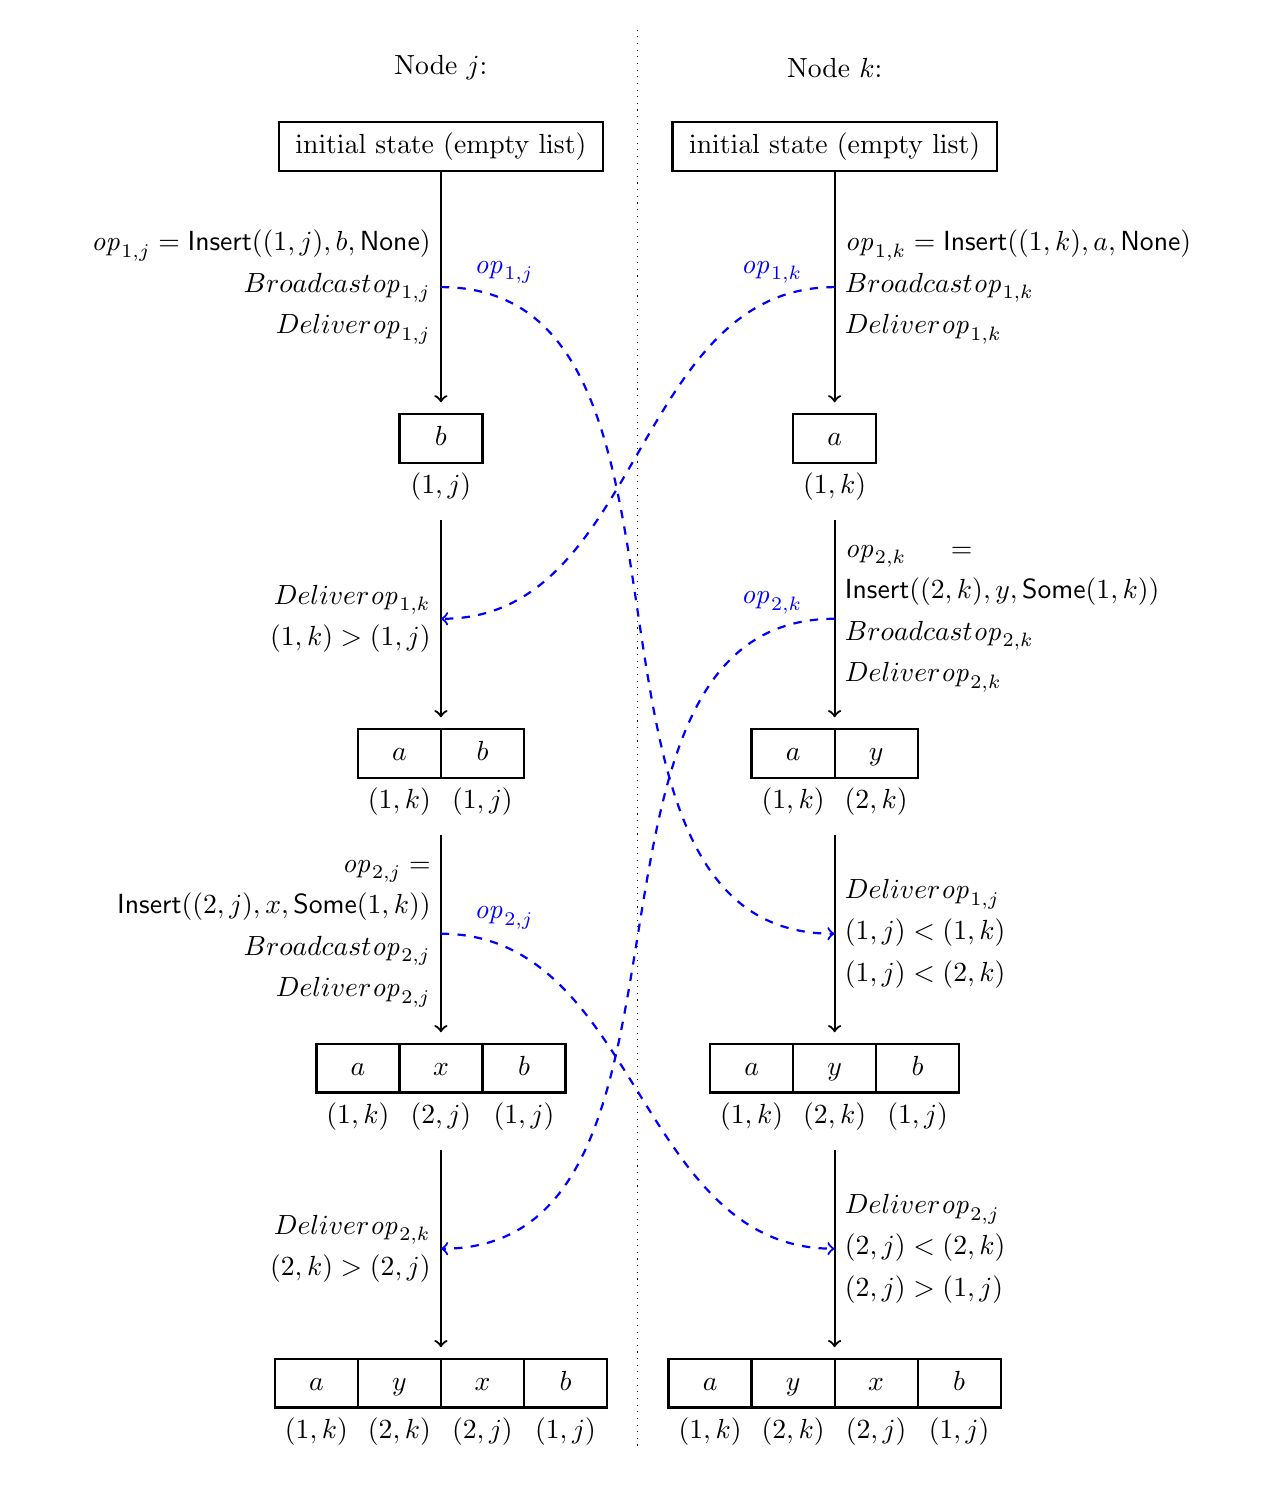
\begin{tikzpicture}[auto,scale=1.0]
\onehalfspacing
\path [draw,dotted] (2.5,-0.5) -- (2.5,17.5);

\tikzstyle{initstate}=[rectangle,draw,inner xsep=6pt,text height=8pt,text depth=3pt]
\tikzstyle{state}=[matrix,column sep={30pt,between origins}]
\tikzstyle{val}=[draw,anchor=base,minimum width=30pt,text height=8pt,text depth=3pt]
\tikzstyle{oid}=[anchor=base]
\tikzstyle{leftevent}=[left,text width=5cm,text ragged left,midway]
\tikzstyle{rightevent}=[right,text width=5cm,text ragged,midway]
\tikzstyle{every path}=[thick,->]

\node (leftR) at (0,17) {Node $j$:};
\node (left1) at (0,16) [initstate] {initial state (empty list)};
\node (left2) at (0,12) [state] {
    \node [val] {$b$};     \\
    \node [oid] {$(1,j)$}; \\
};
\node (left3) at (0,8) [state] {
    \node [val] {$a$};     & \node [val] {$b$};     \\
    \node [oid] {$(1,k)$}; & \node [oid] {$(1,j)$}; \\
};
\node (left4) at (0,4) [state] {
    \node [val] {$a$};     & \node [val] {$x$};     & \node [val] {$b$};     \\
    \node [oid] {$(1,k)$}; & \node [oid] {$(2,j)$}; & \node [oid] {$(1,j)$}; \\
};
\node (left5) at (0,0) [state] {
    \node [val] {$a$};     & \node [val] {$y$};     & \node [val] {$x$};     & \node [val] {$b$};     \\
    \node [oid] {$(1,k)$}; & \node [oid] {$(2,k)$}; & \node [oid] {$(2,j)$}; & \node [oid] {$(1,j)$}; \\
};

\draw (left1) -- (left2) node (send1j) [leftevent] {
    \hfill $\mathit{op}_{1,j} = \mathsf{Insert}((1, j), b, \mathsf{None})$ \\
    \hfill $\text{Broadcast } \mathit{op}_{1,j}$ \\
    \hfill $\text{Deliver } \mathit{op}_{1,j}$ \\
};
\draw (left2) -- (left3) node (recv1k) [leftevent] {
    \hfill $\text{Deliver } \mathit{op}_{1,k}$ \\
    \hfill $(1,k) > (1,j)$ \\
};
\draw (left3) -- (left4) node (send2j) [leftevent] {
    \hfill $\mathit{op}_{2,j} = \mathsf{Insert}((2, j), x, \mathsf{Some}(1,k))$ \\
    \hfill $\text{Broadcast } \mathit{op}_{2,j}$ \\
    \hfill $\text{Deliver } \mathit{op}_{2,j}$ \\
};
\draw (left4) -- (left5) node (recv2k) [leftevent] {
    \hfill $\text{Deliver } \mathit{op}_{2,k}$ \\
    \hfill $(2,k) > (2,j)$ \\
};

\node (rightR) at (5,17) {Node $k$:};
\node (right1) at (5,16) [initstate] {initial state (empty list)};
\node (right2) at (5,12) [state] {
    \node [val] {$a$};     \\
    \node [oid] {$(1,k)$}; \\
};
\node (right3) at (5,8) [state] {
    \node [val] {$a$};     & \node [val] {$y$};     \\
    \node [oid] {$(1,k)$}; & \node [oid] {$(2,k)$}; \\
};
\node (right4) at (5,4) [state] {
    \node [val] {$a$};     & \node [val] {$y$};     & \node [val] {$b$};     \\
    \node [oid] {$(1,k)$}; & \node [oid] {$(2,k)$}; & \node [oid] {$(1,j)$}; \\
};
\node (right5) at (5,0) [state] {
    \node [val] {$a$};     & \node [val] {$y$};     & \node [val] {$x$};     & \node [val] {$b$};     \\
    \node [oid] {$(1,k)$}; & \node [oid] {$(2,k)$}; & \node [oid] {$(2,j)$}; & \node [oid] {$(1,j)$}; \\
};

\draw (right1) -- (right2) node (send1k) [rightevent] {
    $\mathit{op}_{1,k} = \mathsf{Insert}((1, k), a, \mathsf{None})$ \\
    $\text{Broadcast } \mathit{op}_{1,k}$ \\
    $\text{Deliver } \mathit{op}_{1,k}$ \\
};
\draw (right2) -- (right3) node (send2k) [rightevent] {
    $\mathit{op}_{2,k} = \mathsf{Insert}((2, k), y, \mathsf{Some}(1, k))$ \\
    $\text{Broadcast } \mathit{op}_{2,k}$ \\
    $\text{Deliver } \mathit{op}_{2,k}$ \\
};
\draw (right3) -- (right4) node (recv1j) [rightevent] {
    $\text{Deliver } \mathit{op}_{1,j}$ \\
    $(1,j) < (1,k)$ \\
    $(1,j) < (2,k)$ \\
};
\draw (right4) -- (right5) node (recv2j) [rightevent] {
    $\text{Deliver } \mathit{op}_{2,j}$ \\
    $(2,j) < (2,k)$ \\
    $(2,j) > (1,j)$ \\
};

\begin{scope}[dashed,blue]
    \tikzstyle{every node}=[text centered]
    \draw (send1j.east) to [out=0,in=180] (recv1j.west);
    \draw (send2j.east) to [out=0,in=180] (recv2j.west);
    \draw (send1k.west) to [out=180,in=0] (recv1k.east);
    \draw (send2k.west) to [out=180,in=0] (recv2k.east);
    \node at (0.8,14.4) {$\mathit{op}_{1,j}$};
    \node at (0.8, 6.2) {$\mathit{op}_{2,j}$};
    \node at (4.2,14.4) {$\mathit{op}_{1,k}$};
    \node at (4.2,10.2) {$\mathit{op}_{2,k}$};
\end{scope}
\end{tikzpicture}

\caption{RGA example}\label{fig.two-lists}
\end{figure}


\subsection{An overview of Isabelle}
\label{subsect.an.overview.of.isabelle}

All of our proofs are checked with the Isabelle proof assistant~\cite{DBLP:conf/tphol/WenzelPN08}.
Accordingly, we now provide a brief introduction to the Isabelle logical framework, and to the Isabelle/HOL object logic, so that the reader can easily follow our proofs, and understand our theorem statements.
The interested reader is invited to reference standard tutorial material on Isabelle, for a more in-depth introduction to the system~\cite{DBLP:books/sp/NipkowK14}.

Isabelle is a logical framework, providing a weak meta-logic---a fragment of intuitionistic higher-order logic---within which object logics may be embedded as theories.
One particular object logic embedding---Isabelle/HOL, a more expressive implementation of Gordon's higher-order logic than that provided by the meta-logic---is the arena in which we formalise our proof of convergence.

% Type system

Isabelle/HOL is a strictly-typed logic.
The logic's type system resembles that of mainstream functional programming languages, such as Standard ML, OCaml, or Haskell, albeit without the let-polymorphism that each of these languages implement.
\emph{Function types} are written $\tau_1 \Rightarrow \tau_2$, and are inhabited by \emph{total} functions, mapping elements of $\tau_1$ to elements of $\tau_2$.
Here, `total' means that all recursive function definitions must terminate i.e. recurse on some smaller argument, with respect to a well-founded order.
We write $\tau_1 \times \tau_2$ for the \emph{product type} of $\tau_1$ and $\tau_2$, inhabited by pairs of elements of type $\tau_1$ and $\tau_2$, respectively.
In a similar fashion to Standard ML and OCaml, but differing from Haskell, \emph{type operators} are applied to arguments in reverse order.
We therefore write $\tau\ \isa{list}$ and $\tau\ \isa{set}$ for the type of lists of elements of type $\tau$, and the type of mathematical (i.e. potentially infinite) sets of type $\tau$, respectively.
Type variable are written in Greek lowercase, with, $\alpha \Rightarrow \alpha$ denoting the type of a polymorphic identity function, for example.

Isabelle/HOL's term language again contains many features one would typically find in a mainstream functional programming language.
We write $\isa{t} \isa{::} \tau$ for a \emph{type ascription}, constraining the type of the term $\isa{t}$ to the type $\tau$.
We write $\lambda{x}. t$ for an anonymous function mapping an argument $\isa{x}$ to $\isa{t(x)}$, and write the application of term $\isa{t}$ with function type to an argument $\isa{u}$ as $\isa{t\ u}$, as usual.
Terms of list type are introduced using one of two constructors: $\isa{[]}$, or `nil', and $\isa{\#}$, or `cons', which prepends an element to an existing list.
We use $[t_1, \ldots, t_n]$ as syntactic sugar for a list literal, which is desugared into a series of cons applications.
We write $\{\}$ for the empty set, and use usual mathematical notation for set union, disjunction, membership tests, and so on: $\isa{t} \cup \isa{u}$, $\isa{t} \cap \isa{u}$, and $\isa{x} \in \isa{t}$.
Local definitions, within the body of a term, may be made with a let-in construct.

Terms with type $\isa{bool}$ are called \emph{formulae}.
We write $\isa{True}$ and $\isa{False}$ for the logical truthity and falsity constants, respectively.

% Definitions and recursive functions

% Inductive relations

% Formulae, theorem statements

% Proofs

% move into background

\section{High-level proof strategy}
\label{sect.high-level.proof.strategy}

Before embarking on a detailed description of our formal proof of convergence in Isabelle, we provide a higher-level overview of the proof strategy used.

%%%%%%%%%%%%%%%%%%%%%%%%%%%%%%%%%%%%%%%%%%%%%%%%%%%%%%%%%%%%%%%%%%%%%%%%%%%%%%%%
% Convergence
%%%%%%%%%%%%%%%%%%%%%%%%%%%%%%%%%%%%%%%%%%%%%%%%%%%%%%%%%%%%%%%%%%%%%%%%%%%%%%%%

\section{Convergence}
\label{sect.convergence}

\subsection{Our consistency model, and main theorem statement}
\label{subsect.consistency.model.main.theorem.statement}

% move into background?

Distributed systems---by their very nature---include replication and communication between replicas over a network.
Messages passed back and forth between replicas may be delayed, reordered, or lost entirely.
These effects may be caused by networking or other hardware faults, a conscious trade-off in the design of the networking protocol used, or they may simply be an inevitable result of geographic separation between replicas.
As a result, local state changes at any given pair of replicas may progress with differing views of the system's overall shared state.

A natural question to ask of a distributed system, therefore, is whether any two replicas will converge to the same state, and under what conditions that convergence will happen.
A \emph{consistency model} enumerates the criteria under which a distributed system converges, when, and how a replica's view of the system's state is related to the view of any other replica.
Several standard consistency models for distributed systems exist in the literature, with differing strengths and weaknesses.
We discuss three here: \emph{strict (or strong) consistency}, \emph{eventual consistency}, and a variant of the latter called \emph{strong eventual consistency}.

\emph{Strict (or strong) consistency} is a popular consistency model for transactional databases.
Upon a replica updating some subcomponent of the system's shared state, strict consistency guarantees that all other replicas immediately see this update.
This is a strong requirement, and for many distributed systems is often impossible to implement due to physical constraints---notice of updates to the system's shared state may take significant amounts of time to percolate to geographically widely separated replicas, for instance.
Further, in cases where one is able to achieve strict consistency, updates to the system's shared state may require global locks, or some other performance-degrading mechanism deemed unacceptable to the architects of the system.
These problems with strict consistency motivate various relaxed consistency models, including eventual consistency.

\emph{Eventual consistency} is a widely used consistency model in distributed systems, and a relaxation of the strict consistency model.
Many commercially deployed systems, particularly distributed data stores, and vital components of Internet infrastructure, such as the Domain Name System (DNS), use eventual consistency as their consistency model.
Barring no new updates to some subcomponent of the system's shared state, eventual consistency guarantees that at some future point all replicas will agree on the state of that subcomponent.
Naturally, eventual consistency requires a means of addressing conflicts when concurrent updates to the system's state are detected, and different strategies may be deployed, dependending on the requirements of the particular system.
Popular strategies include invoking a user-specified conflict resolution handler upon detection of conflicts, or uniformly applying a \emph{last writer wins} policy to all conflicts.
These strategies are often \emph{ad hoc} and error prone, motivating variants of the consistency model, including strong eventual consistency.

\emph{Strong eventual consistency} is a special case of eventual consistency.
In a strongly eventual consistent system, the operations that a replica may use to modify subcomponents of the system's shared global state are constrained in such a way that pairs of operations naturally commute with each other.
As a result, the system will eventually reach a consistent state, but the potentially error prone process of invoking conflict resolution strategies is no longer needed, as conflicts are impossible to introduce, by construction.
This consistency model is impossible to achieve for many distributed systems, but it is the natural consistency model---and therefore notion of correctness---for Conflict-free Replicated Datatypes, whose operations are guaranteed to commute, as previously described.

In this work, we prove that our Replicated Growable Array implementation possesses this convergence property in an abstract setting.
Our final theorem states that two arbitrary lists of distinct events enriched by an order relation, that satisfy a consistency property defined in terms of a \emph{happens before} relation, converge to the same state.
Formally, we prove:
\\
\begin{isabellebody}
\ \ \ \ \isacommand{theorem} convergence{\isacharcolon}\isanewline
\ \ \ \ \ \ \isakeyword{assumes}\ {\isachardoublequoteopen}set\ xs\ {\isacharequal}\ set\ ys{\isachardoublequoteclose}\isanewline
\ \ \ \ \ \ \ \ \ \ \isakeyword{and}\ {\isachardoublequoteopen}concurrent{\isacharunderscore}ops{\isacharunderscore}commute\ xs{\isachardoublequoteclose}\ \isakeyword{and}\ {\isachardoublequoteopen}concurrent{\isacharunderscore}ops{\isacharunderscore}commute\ ys{\isachardoublequoteclose}\isanewline
\ \ \ \ \ \ \ \ \ \ \isakeyword{and}\ {\isachardoublequoteopen}distinct\ xs{\isachardoublequoteclose}\ \isakeyword{and}\ {\isachardoublequoteopen}distinct\ ys{\isachardoublequoteclose}\isanewline
\ \ \ \ \ \ \ \ \ \ \isakeyword{and}\ {\isachardoublequoteopen}hb{\isacharunderscore}consistent\ xs{\isachardoublequoteclose}\ \isakeyword{and}\ {\isachardoublequoteopen}hb{\isacharunderscore}consistent\ ys{\isachardoublequoteclose}\isanewline
\ \ \ \ \ \ \ \ \isakeyword{shows}\ {\isachardoublequoteopen}apply{\isacharunderscore}operations\ xs\ {\isacharequal}\ apply{\isacharunderscore}operations\ ys{\isachardoublequoteclose}\isanewline
\end{isabellebody}
That is, suppose $\isa{xs}$ and $\isa{ys}$ are two arbitrary list of distinct events, that contain the same set of elements, but are ordered in a way that respects our \emph{happens before} relation---that is, so earlier elements in the list all \emph{happen before} later ones.
Suppose also that any two events in $\isa{xs}$ (respectively, $\isa{ys}$) that happen concurrently, per our \emph{happens before} relation, have a commuting property on states.
Then the final state one obtains by applying

Let $\mathit{Events}$ be the set of events enriched with a preorder $\prec$. We
write $\isa{x} \prec \isa{y}$ and say that the event \isa{x} \emph{happens
before} the event \isa{y}.  Moreover we assume that there exists an
interpretation partial function $\langle\_\rangle$ that maps events to
\emph{operations}, which are \emph{state transformers} on a set of states
$\Sigma$.  This is implemented in Isabelle by the following \textbf{locale}
statement.

\begin{isabellebody}
  \isanewline
\isacommand{locale}\isamarkupfalse%
\ happens{\isacharunderscore}before\ {\isacharequal}\ preorder\ hb{\isacharunderscore}weak\ hb\isanewline
\ \ \isakeyword{for}\ hb{\isacharunderscore}weak\ {\isacharcolon}{\isacharcolon}\ {\isachardoublequoteopen}{\isacharprime}a\ {\isasymRightarrow}\ {\isacharprime}a\ {\isasymRightarrow}\ bool{\isachardoublequoteclose}\ \ {\isacharparenleft}\isakeyword{infix}\ {\isachardoublequoteopen}{\isasympreceq}{\isachardoublequoteclose}\ {\isadigit{5}}{\isadigit{0}}{\isacharparenright}\isanewline
\ \ \isakeyword{and}\ hb\ {\isacharcolon}{\isacharcolon}\ {\isachardoublequoteopen}{\isacharprime}a\ {\isasymRightarrow}\ {\isacharprime}a\ {\isasymRightarrow}\ bool{\isachardoublequoteclose}\ \ \ \ \ \ \ {\isacharparenleft}\isakeyword{infix}\ {\isachardoublequoteopen}{\isasymprec}{\isachardoublequoteclose}\ {\isadigit{5}}{\isadigit{0}}{\isacharparenright}\ {\isacharplus}\isanewline
\ \ \isakeyword{fixes}\ interp\ {\isacharcolon}{\isacharcolon}\ {\isachardoublequoteopen}{\isacharprime}a\ {\isasymRightarrow}\ {\isacharprime}b\ {\isasymrightharpoonup}\ {\isacharprime}b{\isachardoublequoteclose}\ {\isacharparenleft}{\isachardoublequoteopen}{\isasymlangle}{\isacharunderscore}{\isasymrangle}{\isachardoublequoteclose}\ {\isacharbrackleft}{\isadigit{0}}{\isacharbrackright}\ {\isadigit{1}}{\isadigit{0}}{\isadigit{0}}{\isadigit{0}}{\isacharparenright}\isanewline
\end{isabellebody}

We say that two events (or operations) $x$ and $y$ are \emph{concurrent}
whenever one does not happens before the other, that is, $\neg (\isa{x} \prec
\isa{y})$ and $\neg (\isa{y} \prec \isa{x})$.

\begin{isabellebody}
  \isanewline
\isacommand{definition}\isamarkupfalse%
\ concurrent\ {\isacharcolon}{\isacharcolon}\ {\isachardoublequoteopen}{\isacharprime}a\ {\isasymRightarrow}\ {\isacharprime}a\ {\isasymRightarrow}\ bool{\isachardoublequoteclose}\ {\isacharparenleft}\isakeyword{infix}\ {\isachardoublequoteopen}{\isasymparallel}{\isachardoublequoteclose}\ {\isadigit{5}}{\isadigit{0}}{\isacharparenright}\ \isakeyword{where}\isanewline
\ \ {\isachardoublequoteopen}x\ {\isasymparallel}\ y\ {\isasymequiv}\ {\isasymnot}\ {\isacharparenleft}x\ {\isasymprec}\ y{\isacharparenright}\ {\isasymand}\ {\isasymnot}\ {\isacharparenleft}y\ {\isasymprec}\ x{\isacharparenright}{\isachardoublequoteclose}\isanewline
\end{isabellebody}

A list of events \isa{xs} is \emph{hb-consistent}, or simply \emph{consistent},
whenever for any element \isa{y}, it is not the case that \isa{y} happens
before \isa{x} for all \isa{x} that appears before \isa{y} in the list. That
is, \isa{x} and \isa{y} are either concurrent or \isa{x} happens before
\isa{y}.  This is implemented in Isabelle by an inductive predicate.

\begin{isabellebody}
  \isanewline
\isacommand{inductive}\isamarkupfalse%
\ hb{\isacharunderscore}consistent\ {\isacharcolon}{\isacharcolon}\ {\isachardoublequoteopen}{\isacharprime}a\ list\ {\isasymRightarrow}\ bool{\isachardoublequoteclose}\ \isakeyword{where}\isanewline
\ \ {\isachardoublequoteopen}hb{\isacharunderscore}consistent\ {\isacharbrackleft}{\isacharbrackright}{\isachardoublequoteclose}\ {\isacharbar}\isanewline
\ \ {\isachardoublequoteopen}{\isasymlbrakk}\ hb{\isacharunderscore}consistent\ xs{\isacharsemicolon}\ {\isasymforall}x\ {\isasymin}\ set\ xs{\isachardot}\ {\isasymnot}\ y\ {\isasymprec}\ x\ {\isasymrbrakk}\ {\isasymLongrightarrow}\ hb{\isacharunderscore}consistent\ {\isacharparenleft}xs\ {\isacharat}\ {\isacharbrackleft}y{\isacharbrackright}{\isacharparenright}{\isachardoublequoteclose}\isanewline
\end{isabellebody}

Additionally, we say that concurrent operations commute in a list \isa{xs}
whenever for all concurrent events \isa{x} and \isa{y} in the list \isa{xs},
the Kleisli arrow composition of their operations commute $\langle \isa{x}
\rangle \rhd \langle \isa{y} \rangle = \langle \isa{y} \rangle \rhd \langle
\isa{x} \rangle$.

\begin{isabellebody}
  \isanewline
\isacommand{definition}\isamarkupfalse%
\ concurrent{\isacharunderscore}ops{\isacharunderscore}commute\ {\isacharcolon}{\isacharcolon}\ {\isachardoublequoteopen}{\isacharprime}a\ list\ {\isasymRightarrow}\ bool{\isachardoublequoteclose}\ \isakeyword{where}\isanewline
\ \ {\isachardoublequoteopen}concurrent{\isacharunderscore}ops{\isacharunderscore}commute\ xs\ {\isasymequiv}
\ {\isasymforall}x\ y{\isachardot}\ {\isacharbraceleft}x{\isacharcomma}\ y{\isacharbraceright}\ {\isasymsubseteq}\ set\ xs\ {\isasymlongrightarrow}\ x\ {\isasymparallel}\ y\ {\isasymlongrightarrow}\ {\isasymlangle}x{\isasymrangle}{\isasymrhd}{\isasymlangle}y{\isasymrangle}\ {\isacharequal}\ {\isasymlangle}y{\isasymrangle}{\isasymrhd}{\isasymlangle}x{\isasymrangle}{\isachardoublequoteclose}\isanewline

\isacommand{definition}\isamarkupfalse%
\ kleisli\ {\isacharcolon}{\isacharcolon}\ {\isachardoublequoteopen}{\isacharparenleft}{\isacharprime}b\ {\isasymRightarrow}\ {\isacharprime}b\ option{\isacharparenright}\ {\isasymRightarrow}\ {\isacharparenleft}{\isacharprime}b\ {\isasymRightarrow}\ {\isacharprime}b\ option{\isacharparenright}\ {\isasymRightarrow}\ {\isacharparenleft}{\isacharprime}b\ {\isasymRightarrow}\ {\isacharprime}b\ option{\isacharparenright}{\isachardoublequoteclose}\ {\isacharparenleft}\isakeyword{infixr}\ {\isachardoublequoteopen}{\isasymrhd}{\isachardoublequoteclose}\ {\isadigit{6}}{\isadigit{5}}{\isacharparenright}\ \isakeyword{where}\isanewline
\ \ {\isachardoublequoteopen}f\ {\isasymrhd}\ g\ {\isasymequiv}\ {\isasymlambda}x{\isachardot}\ f\ x\ {\isasymbind}\ {\isacharparenleft}{\isasymlambda}fx{\isachardot}\ g\ fx{\isacharparenright}{\isachardoublequoteclose}\isanewline
\end{isabellebody}

Let \isa{xs} be a list of events, \isa{apply-operations\ xs} is the state
transformer equivalent of applying in order each operation $\langle \isa{x}
\rangle$ for events \isa{x} in the list.  In other words, it is the fold of
the Kleisli arrow composition on the associated list of operations.

\begin{isabellebody}
  \isanewline
\isacommand{definition}\isamarkupfalse%
\ apply{\isacharunderscore}operations\ {\isacharcolon}{\isacharcolon}\ {\isachardoublequoteopen}{\isacharprime}a\ list\ {\isasymRightarrow}\ {\isacharprime}b\ {\isasymrightharpoonup}\ {\isacharprime}b{\isachardoublequoteclose}\ \isakeyword{where}\isanewline
\ \ {\isachardoublequoteopen}apply{\isacharunderscore}operations\ es\ s\ {\isasymequiv}\ {\isacharparenleft}foldl\ {\isacharparenleft}op\ {\isasymrhd}{\isacharparenright}\ Some\ {\isacharparenleft}map\ interp\ es{\isacharparenright}{\isacharparenright}\ s{\isachardoublequoteclose}\isanewline
\end{isabellebody}

\begin{isabellebody}
\isacommand{lemma}\isamarkupfalse%
\ concurrent{\isacharunderscore}ops{\isacharunderscore}commute{\isacharunderscore}concurrent{\isacharunderscore}set{\isacharcolon}\isanewline
\ \ \isakeyword{assumes}\ {\isachardoublequoteopen}concurrent{\isacharunderscore}ops{\isacharunderscore}commute\ {\isacharparenleft}prefix{\isacharat}suffix{\isacharat}{\isacharbrackleft}x{\isacharbrackright}{\isacharparenright}{\isachardoublequoteclose}\isanewline
\ \ \ \ \ \ \ \ \ \ {\isachardoublequoteopen}concurrent{\isacharunderscore}set\ x\ suffix{\isachardoublequoteclose}\isanewline
\ \ \ \ \ \ \ \ \ \ {\isachardoublequoteopen}distinct\ {\isacharparenleft}prefix\ {\isacharat}\ x\ {\isacharhash}\ suffix{\isacharparenright}{\isachardoublequoteclose}\isanewline
\ \ \isakeyword{shows}\ \ \ {\isachardoublequoteopen}apply{\isacharunderscore}operations\ {\isacharparenleft}prefix\ {\isacharat}\ suffix\ {\isacharat}\ {\isacharbrackleft}x{\isacharbrackright}{\isacharparenright}\ {\isacharequal}\ apply{\isacharunderscore}operations\ {\isacharparenleft}prefix\ {\isacharat}\ x\ {\isacharhash}\ suffix{\isacharparenright}{\isachardoublequoteclose}\isanewline
\end{isabellebody}

We can now formally state the abstract convergence theorem: two consistent list
of distinct events in which concurrent operations commute that have the same
set of elements yield the same state transformer.

\begin{isabellebody}
  \isanewline
\isacommand{theorem}\isamarkupfalse%
\ \ convergence{\isacharcolon}\isanewline
\ \ \isakeyword{assumes}\ {\isachardoublequoteopen}set\ xs\ {\isacharequal}\ set\ ys{\isachardoublequoteclose}\isanewline
\ \ \ \ \ \ \ \ \ \ {\isachardoublequoteopen}concurrent{\isacharunderscore}ops{\isacharunderscore}commute\ xs{\isachardoublequoteclose}\isanewline
\ \ \ \ \ \ \ \ \ \ {\isachardoublequoteopen}concurrent{\isacharunderscore}ops{\isacharunderscore}commute\ ys{\isachardoublequoteclose}\isanewline
\ \ \ \ \ \ \ \ \ \ {\isachardoublequoteopen}distinct\ xs{\isachardoublequoteclose}\isanewline
\ \ \ \ \ \ \ \ \ \ {\isachardoublequoteopen}distinct\ ys{\isachardoublequoteclose}\isanewline
\ \ \ \ \ \ \ \ \ \ {\isachardoublequoteopen}hb{\isacharunderscore}consistent\ xs{\isachardoublequoteclose}\isanewline
\ \ \ \ \ \ \ \ \ \ {\isachardoublequoteopen}hb{\isacharunderscore}consistent\ ys{\isachardoublequoteclose}\isanewline
\ \ \isakeyword{shows}\ \ \ {\isachardoublequoteopen}apply{\isacharunderscore}operations\ xs\ {\isacharequal}\ apply{\isacharunderscore}operations\ ys{\isachardoublequoteclose}\isanewline
\end{isabellebody}

The entire proof is shown in Figure~\ref{fig.convergence}.  The proof follows
by induction on \isa{xs}. The empty list case is immediate. Assuming the
property for \isa{xs}, we prove the case when a new event \isa{x} is added to
the end of \isa{xs}, that is, $\isa{xs}@[\isa{x}]$. Since both lists have the
same elements, one can split \isa{ys} such that \isa{ys = prefix@x@suffix} for
some suitable lists \isa{prefix} and \isa{suffix}. Moreover, all the events in
the set of \isa{suffix} is concurrent to \isa{x}. By the induction hypothesis,
\isa{apply-operations\ xs $=$ apply-operations\ (prefix $@$ suffix)}. Then
\begin{align*}
  \isa{apply-operations}\ (\isa{xs}@[\isa{x}])
  &= \langle\isa{x}\rangle\ (\isa{apply-operations}\ \isa{xs}) \\
  &= \langle\isa{x}\rangle\ (\isa{apply-operations}\ (\isa{prefix}@\isa{suffix}))\\
  &= \isa{apply-operations} (\isa{prefix}@\isa{suffix}@\isa{x}) \\
  &= \isa{apply-operations} (\isa{prefix}@\isa{x@\isa{suffix}}) \\
  &= \isa{apply-operations}\ ys.
\end{align*}


\begin{figure}
  \raggedright
  \begin{isabellebody}
\isanewline
\isacommand{theorem}\isamarkupfalse%
\ \ convergence{\isacharcolon}\isanewline
\ \ \isakeyword{assumes}\ {\isachardoublequoteopen}set\ xs\ {\isacharequal}\ set\ ys{\isachardoublequoteclose}\isanewline
\ \ \ \ \ \ \ \ \ \ {\isachardoublequoteopen}concurrent{\isacharunderscore}ops{\isacharunderscore}commute\ xs{\isachardoublequoteclose}\isanewline
\ \ \ \ \ \ \ \ \ \ {\isachardoublequoteopen}concurrent{\isacharunderscore}ops{\isacharunderscore}commute\ ys{\isachardoublequoteclose}\isanewline
\ \ \ \ \ \ \ \ \ \ {\isachardoublequoteopen}distinct\ xs{\isachardoublequoteclose}\isanewline
\ \ \ \ \ \ \ \ \ \ {\isachardoublequoteopen}distinct\ ys{\isachardoublequoteclose}\isanewline
\ \ \ \ \ \ \ \ \ \ {\isachardoublequoteopen}hb{\isacharunderscore}consistent\ xs{\isachardoublequoteclose}\isanewline
\ \ \ \ \ \ \ \ \ \ {\isachardoublequoteopen}hb{\isacharunderscore}consistent\ ys{\isachardoublequoteclose}\isanewline
\ \ \isakeyword{shows}\ \ \ {\isachardoublequoteopen}apply{\isacharunderscore}operations\ xs\ {\isacharequal}\ apply{\isacharunderscore}operations\ ys{\isachardoublequoteclose}\isanewline
%
\isacommand{using}\isamarkupfalse%
\ assms\ \isacommand{proof}\isamarkupfalse%
{\isacharparenleft}induction\ xs\ arbitrary{\isacharcolon}\ ys\ rule{\isacharcolon}\ rev{\isacharunderscore}induct{\isacharcomma}\ simp{\isacharparenright}\isanewline
\ \ \isacommand{case}\isamarkupfalse%
\ assms{\isacharcolon}\ {\isacharparenleft}snoc\ x\ xs{\isacharparenright}\isanewline
\ \ \isacommand{then}\isamarkupfalse%
\ \isacommand{obtain}\isamarkupfalse%
\ prefix\ suffix\ \isakeyword{where}\ ys{\isacharunderscore}split{\isacharcolon}\ {\isachardoublequoteopen}ys\ {\isacharequal}\ prefix\ {\isacharat}\ x\ {\isacharhash}\ suffix\ {\isasymand}\ concurrent{\isacharunderscore}set\ x\ suffix{\isachardoublequoteclose}\isanewline
\ \ \ \ \isacommand{using}\isamarkupfalse%
\ hb{\isacharunderscore}consistent{\isacharunderscore}prefix{\isacharunderscore}suffix{\isacharunderscore}exists\ \isacommand{by}\isamarkupfalse%
\ fastforce\isanewline
\ \ \isacommand{moreover}\isamarkupfalse%
\ \isacommand{hence}\isamarkupfalse%
\ {\isacharasterisk}{\isacharcolon}\ {\isachardoublequoteopen}distinct\ {\isacharparenleft}prefix\ {\isacharat}\ suffix{\isacharparenright}{\isachardoublequoteclose}\ {\isachardoublequoteopen}hb{\isacharunderscore}consistent\ xs{\isachardoublequoteclose}\isanewline
\ \ \ \ \isacommand{using}\isamarkupfalse%
\ assms\ \isacommand{by}\isamarkupfalse%
\ auto\isanewline
\ \ \isacommand{moreover}\isamarkupfalse%
\ \isacommand{{\isacharbraceleft}}\isamarkupfalse%
\isanewline
\ \ \ \ \isacommand{have}\isamarkupfalse%
\ {\isachardoublequoteopen}hb{\isacharunderscore}consistent\ prefix{\isachardoublequoteclose}\ {\isachardoublequoteopen}hb{\isacharunderscore}consistent\ suffix{\isachardoublequoteclose}\isanewline
\ \ \ \ \ \ \isacommand{using}\isamarkupfalse%
\ ys{\isacharunderscore}split\ assms\ hb{\isacharunderscore}consistent{\isacharunderscore}append{\isacharunderscore}D{\isadigit{2}}\ hb{\isacharunderscore}consistent{\isacharunderscore}append{\isacharunderscore}elim{\isacharunderscore}ConsD\ \isacommand{by}\isamarkupfalse%
\ blast{\isacharplus}\isanewline
\ \ \ \ \isacommand{hence}\isamarkupfalse%
\ {\isachardoublequoteopen}hb{\isacharunderscore}consistent\ {\isacharparenleft}prefix\ {\isacharat}\ suffix{\isacharparenright}{\isachardoublequoteclose}\isanewline
\ \ \ \ \ \ \isacommand{by}\isamarkupfalse%
\ {\isacharparenleft}metis\ assms{\isacharparenleft}{\isadigit{8}}{\isacharparenright}\ hb{\isacharunderscore}consistent{\isacharunderscore}append\ hb{\isacharunderscore}consistent{\isacharunderscore}append{\isacharunderscore}porder\ list{\isachardot}set{\isacharunderscore}intros{\isacharparenleft}{\isadigit{2}}{\isacharparenright}\ ys{\isacharunderscore}split{\isacharparenright}\isanewline
\ \ \isacommand{{\isacharbraceright}}\isamarkupfalse%
\isanewline
\ \ \isacommand{moreover}\isamarkupfalse%
\ \isacommand{have}\isamarkupfalse%
\ {\isacharasterisk}{\isacharasterisk}{\isacharcolon}\ {\isachardoublequoteopen}concurrent{\isacharunderscore}ops{\isacharunderscore}commute\ {\isacharparenleft}prefix\ {\isacharat}\ suffix\ {\isacharat}\ {\isacharbrackleft}x{\isacharbrackright}{\isacharparenright}{\isachardoublequoteclose}\isanewline
\ \ \ \ \isacommand{using}\isamarkupfalse%
\ assms\ ys{\isacharunderscore}split\ \isacommand{by}\isamarkupfalse%
\ {\isacharparenleft}clarsimp\ simp{\isacharcolon}\ concurrent{\isacharunderscore}ops{\isacharunderscore}commute{\isacharunderscore}def{\isacharparenright}\isanewline
\ \ \isacommand{moreover}\isamarkupfalse%
\ \isacommand{hence}\isamarkupfalse%
\ {\isachardoublequoteopen}concurrent{\isacharunderscore}ops{\isacharunderscore}commute\ {\isacharparenleft}prefix\ {\isacharat}\ suffix{\isacharparenright}{\isachardoublequoteclose}\isanewline
\ \ \ \ \isacommand{by}\isamarkupfalse%
\ {\isacharparenleft}force\ simp\ del{\isacharcolon}\ append{\isacharunderscore}assoc\ simp\ add{\isacharcolon}\ append{\isacharunderscore}assoc{\isacharbrackleft}symmetric{\isacharbrackright}{\isacharparenright}\isanewline
\ \ \isacommand{ultimately}\isamarkupfalse%
\ \isacommand{have}\isamarkupfalse%
\ {\isachardoublequoteopen}apply{\isacharunderscore}operations\ xs\ {\isacharequal}\ apply{\isacharunderscore}operations\ {\isacharparenleft}prefix{\isacharat}suffix{\isacharparenright}{\isachardoublequoteclose}\isanewline
\ \ \ \ \isacommand{using}\isamarkupfalse%
\ assms\ \isacommand{by}\isamarkupfalse%
\ simp\ {\isacharparenleft}metis\ Diff{\isacharunderscore}insert{\isacharunderscore}absorb\ Un{\isacharunderscore}iff\ {\isacharasterisk}\ concurrent{\isacharunderscore}ops{\isacharunderscore}commute{\isacharunderscore}appendD\ set{\isacharunderscore}append{\isacharparenright}\isanewline
\ \ \isacommand{moreover}\isamarkupfalse%
\ \isacommand{have}\isamarkupfalse%
\ {\isachardoublequoteopen}apply{\isacharunderscore}operations\ {\isacharparenleft}prefix{\isacharat}suffix\ {\isacharat}\ {\isacharbrackleft}x{\isacharbrackright}{\isacharparenright}\ {\isacharequal}\ apply{\isacharunderscore}operations\ {\isacharparenleft}prefix{\isacharat}x\ {\isacharhash}\ suffix{\isacharparenright}{\isachardoublequoteclose}\isanewline
\ \ \ \ \isacommand{using}\isamarkupfalse%
\ ys{\isacharunderscore}split\ assms\ {\isacharasterisk}{\isacharasterisk}\ concurrent{\isacharunderscore}ops{\isacharunderscore}commute{\isacharunderscore}concurrent{\isacharunderscore}set\ \isacommand{by}\isamarkupfalse%
\ force\isanewline
\ \ \isacommand{ultimately}\isamarkupfalse%
\ \isacommand{show}\isamarkupfalse%
\ {\isacharquery}case\isanewline
\ \ \ \ \isacommand{using}\isamarkupfalse%
\ ys{\isacharunderscore}split\ \isacommand{by}\isamarkupfalse%
\ {\isacharparenleft}force\ simp{\isacharcolon}\ append{\isacharunderscore}assoc{\isacharbrackleft}symmetric{\isacharbrackright}\ simp\ del{\isacharcolon}\ append{\isacharunderscore}assoc{\isacharparenright}\isanewline
\isacommand{qed}\isamarkupfalse%
  \end{isabellebody}
  \caption{Proof of convergence theorem in Isar.}
  \label{fig.convergence}
\end{figure}


%%%%%%%%%%%%%%%%%%%%%%%%%%%%%%%%%%%%%%%%%%%%%%%%%%%%%%%%%%%%%%%%%%%%%%%%%%%%%%%%
% Network
%%%%%%%%%%%%%%%%%%%%%%%%%%%%%%%%%%%%%%%%%%%%%%%%%%%%%%%%%%%%%%%%%%%%%%%%%%%%%%%%

\section{Network}
\label{sect.network}

\begin{isabellebody}
\isanewline
\isacommand{locale}\isamarkupfalse%
\ node{\isacharunderscore}histories\ {\isacharequal}\ \isanewline
\ \ \isakeyword{fixes}\ history\ {\isacharcolon}{\isacharcolon}\ {\isachardoublequoteopen}nat\ {\isasymRightarrow}\ {\isacharprime}a\ list{\isachardoublequoteclose}\isanewline
\ \ \isakeyword{assumes}\ histories{\isacharunderscore}distinct{\isacharcolon}\ {\isachardoublequoteopen}distinct\ {\isacharparenleft}history\ i{\isacharparenright}{\isachardoublequoteclose}\isanewline
\end{isabellebody}

\begin{isabellebody}
\isanewline
\isacommand{definition}\isamarkupfalse%
\ {\isacharparenleft}\isakeyword{in}\ node{\isacharunderscore}histories{\isacharparenright}\ history{\isacharunderscore}order\ {\isacharcolon}{\isacharcolon}\ {\isachardoublequoteopen}{\isacharprime}a\ {\isasymRightarrow}\ nat\ {\isasymRightarrow}\ {\isacharprime}a\ {\isasymRightarrow}\ bool{\isachardoublequoteclose}\ {\isacharparenleft}{\isachardoublequoteopen}{\isacharunderscore}{\isacharslash}\ {\isasymsqsubset}\isactrlsup {\isacharunderscore}{\isacharslash}\ {\isacharunderscore}{\isachardoublequoteclose}\ {\isacharbrackleft}{\isadigit{5}}{\isadigit{0}}{\isacharcomma}{\isadigit{1}}{\isadigit{0}}{\isadigit{0}}{\isadigit{0}}{\isacharcomma}{\isadigit{5}}{\isadigit{0}}{\isacharbrackright}{\isadigit{5}}{\isadigit{0}}{\isacharparenright}\ \isakeyword{where}\isanewline
\ \ {\isachardoublequoteopen}x\ {\isasymsqsubset}\isactrlsup i\ z\ {\isasymequiv}\ {\isasymexists}xs\ ys\ zs{\isachardot}\ xs{\isacharat}x{\isacharhash}ys{\isacharat}z{\isacharhash}zs\ {\isacharequal}\ history\ i{\isachardoublequoteclose}\isanewline
\end{isabellebody}

\begin{isabellebody}
\isanewline
\isacommand{definition}\isamarkupfalse%
\ {\isacharparenleft}\isakeyword{in}\ node{\isacharunderscore}histories{\isacharparenright}\ prefix{\isacharunderscore}of{\isacharunderscore}node{\isacharunderscore}history\ {\isacharcolon}{\isacharcolon}\ {\isachardoublequoteopen}{\isacharprime}a\ list\ {\isasymRightarrow}\ nat\ {\isasymRightarrow}\ bool{\isachardoublequoteclose}\ {\isacharparenleft}\isakeyword{infix}\ {\isachardoublequoteopen}prefix\ of{\isachardoublequoteclose}\ {\isadigit{5}}{\isadigit{0}}{\isacharparenright}\ \isakeyword{where}\isanewline
\ \ {\isachardoublequoteopen}xs\ prefix\ of\ i\ {\isasymequiv}\ {\isasymexists}ys{\isachardot}\ xs{\isacharat}ys\ {\isacharequal}\ history\ i{\isachardoublequoteclose}\isanewline
\isanewline
\end{isabellebody}

\begin{isabellebody}
\isanewline
\isacommand{datatype}\isamarkupfalse%
\ {\isacharprime}a\ event\isanewline
\ \ {\isacharequal}\ Broadcast\ {\isacharprime}a\isanewline
\ \ {\isacharbar}\ Deliver\ {\isacharprime}a\isanewline
\isanewline
\end{isabellebody}


\begin{isabellebody}
\isanewline
\isacommand{locale}\isamarkupfalse%
\ network\ {\isacharequal}\ node{\isacharunderscore}histories\ history\ \isakeyword{for}\ history\ {\isacharcolon}{\isacharcolon}\ {\isachardoublequoteopen}nat\ {\isasymRightarrow}\ {\isacharprime}a\ event\ list{\isachardoublequoteclose}\ {\isacharplus}\isanewline
\ \ \isakeyword{assumes}\ broadcast{\isacharunderscore}before{\isacharunderscore}delivery{\isacharcolon}\ {\isachardoublequoteopen}Deliver\ m\ {\isasymin}\ set\ {\isacharparenleft}history\ i{\isacharparenright}\ {\isasymLongrightarrow}\ {\isasymexists}j{\isachardot}\ Broadcast\ m\ {\isasymsqsubset}\isactrlsup j\ Deliver\ m{\isachardoublequoteclose}\isanewline
\ \ \isakeyword{and}\ deliver{\isacharunderscore}locally{\isacharcolon}\ {\isachardoublequoteopen}Broadcast\ m\ {\isasymin}\ set\ {\isacharparenleft}history\ i{\isacharparenright}\ {\isasymLongrightarrow}\ Broadcast\ m\ {\isasymsqsubset}\isactrlsup i\ Deliver\ m{\isachardoublequoteclose}\isanewline
\ \ \isakeyword{and}\ broadcasts{\isacharunderscore}unique{\isacharcolon}\ {\isachardoublequoteopen}i\ {\isasymnoteq}\ j\ {\isasymLongrightarrow}\ Broadcast\ m\ {\isasymin}\ set\ {\isacharparenleft}history\ i{\isacharparenright}\ {\isasymLongrightarrow}\ Broadcast\ m\ {\isasymnotin}\ set\ {\isacharparenleft}history\ j{\isacharparenright}{\isachardoublequoteclose}\isanewline
\end{isabellebody}

\begin{isabellebody}
\isanewline
\isacommand{inductive}\isamarkupfalse%
\ {\isacharparenleft}\isakeyword{in}\ network{\isacharparenright}\ hb\ {\isacharcolon}{\isacharcolon}\ {\isachardoublequoteopen}{\isacharprime}a\ {\isasymRightarrow}\ {\isacharprime}a\ {\isasymRightarrow}\ bool{\isachardoublequoteclose}\ \isakeyword{where}\isanewline
\ \ {\isachardoublequoteopen}{\isasymlbrakk}\ Broadcast\ m{\isadigit{1}}\ {\isasymsqsubset}\isactrlsup i\ Broadcast\ m{\isadigit{2}}\ {\isasymrbrakk}\ {\isasymLongrightarrow}\ hb\ m{\isadigit{1}}\ m{\isadigit{2}}{\isachardoublequoteclose}\ {\isacharbar}\isanewline
\ \ {\isachardoublequoteopen}{\isasymlbrakk}\ Deliver\ m{\isadigit{1}}\ {\isasymsqsubset}\isactrlsup i\ Broadcast\ m{\isadigit{2}}\ {\isasymrbrakk}\ {\isasymLongrightarrow}\ hb\ m{\isadigit{1}}\ m{\isadigit{2}}{\isachardoublequoteclose}\ {\isacharbar}\isanewline
\ \ {\isachardoublequoteopen}{\isasymlbrakk}\ hb\ m{\isadigit{1}}\ m{\isadigit{2}}{\isacharsemicolon}\ hb\ m{\isadigit{2}}\ m{\isadigit{3}}\ {\isasymrbrakk}\ {\isasymLongrightarrow}\ hb\ m{\isadigit{1}}\ m{\isadigit{3}}{\isachardoublequoteclose}\isanewline
\ \ \isanewline
\end{isabellebody}

\begin{isabellebody}
\isanewline
\isacommand{locale}\isamarkupfalse%
\ causal{\isacharunderscore}network\ {\isacharequal}\ network\ {\isacharplus}\isanewline
\ \ \isakeyword{assumes}\ causal{\isacharunderscore}delivery{\isacharcolon}\ {\isachardoublequoteopen}Deliver\ m{\isadigit{2}}\ {\isasymin}\ set\ {\isacharparenleft}history\ j{\isacharparenright}\ {\isasymLongrightarrow}\ hb\ m{\isadigit{1}}\ m{\isadigit{2}}\ {\isasymLongrightarrow}\ Deliver\ m{\isadigit{1}}\ {\isasymsqsubset}\isactrlsup j\ Deliver\ m{\isadigit{2}}{\isachardoublequoteclose}\isanewline
\isanewline
\end{isabellebody}

\begin{isabellebody}
\isanewline
\isacommand{definition}\isamarkupfalse%
\ {\isacharparenleft}\isakeyword{in}\ network{\isacharparenright}\ node{\isacharunderscore}deliver{\isacharunderscore}messages\ {\isacharcolon}{\isacharcolon}\ {\isachardoublequoteopen}{\isacharprime}a\ event\ list\ {\isasymRightarrow}\ {\isacharprime}a\ list{\isachardoublequoteclose}\ \isakeyword{where}\isanewline
\ \ {\isachardoublequoteopen}node{\isacharunderscore}deliver{\isacharunderscore}messages\ cs\ {\isasymequiv}\ List{\isachardot}map{\isacharunderscore}filter\ {\isacharparenleft}{\isasymlambda}e{\isachardot}\ case\ e\ of\ Deliver\ m\ {\isasymRightarrow}\ Some\ m\ {\isacharbar}\ {\isacharunderscore}\ {\isasymRightarrow}\ None{\isacharparenright}\ cs{\isachardoublequoteclose}\isanewline
\end{isabellebody}

\begin{isabellebody}
\isanewline
\isacommand{lemma}\isamarkupfalse%
\ {\isacharparenleft}\isakeyword{in}\ causal{\isacharunderscore}network{\isacharparenright}\isanewline
\ \ \isakeyword{shows}\ {\isachardoublequoteopen}hb{\isachardot}hb{\isacharunderscore}consistent\ {\isacharparenleft}node{\isacharunderscore}deliver{\isacharunderscore}messages\ {\isacharparenleft}history\ i{\isacharparenright}{\isacharparenright}{\isachardoublequoteclose}\isanewline
\end{isabellebody}

%%%%%%%%%%%%%%%%%%%%%%%%%%%%%%%%%%%%%%%%%%%%%%%%%%%%%%%%%%%%%%%%%%%%%%%%%%%%%%%%
% RGA
%%%%%%%%%%%%%%%%%%%%%%%%%%%%%%%%%%%%%%%%%%%%%%%%%%%%%%%%%%%%%%%%%%%%%%%%%%%%%%%%

\section{Replicated Growable Array}
\label{sect.rga}

\subsection{Operations}
\label{sect.rga.operations}

\begin{isabellebody}
\isanewline
\isacommand{type{\isacharunderscore}synonym}\isamarkupfalse%
\ {\isacharparenleft}{\isacharprime}id{\isacharcomma}\ {\isacharprime}v{\isacharparenright}\ elt\ {\isacharequal}\ {\isachardoublequoteopen}{\isacharprime}id\ {\isasymtimes}\ {\isacharprime}v\ {\isasymtimes}\ bool{\isachardoublequoteclose}%
\end{isabellebody}


\begin{isabellebody}
\isanewline
\isacommand{fun}\isamarkupfalse%
\ insert{\isacharunderscore}body\ {\isacharcolon}{\isacharcolon}\ {\isachardoublequoteopen}{\isacharparenleft}{\isacharprime}id{\isacharcolon}{\isacharcolon}{\isacharbraceleft}linorder{\isacharbraceright}{\isacharcomma}\ {\isacharprime}v{\isacharparenright}\ elt\ list\ {\isasymRightarrow}\ {\isacharparenleft}{\isacharprime}id{\isacharcomma}\ {\isacharprime}v{\isacharparenright}\ elt\ {\isasymRightarrow}\ {\isacharparenleft}{\isacharprime}id{\isacharcomma}\ {\isacharprime}v{\isacharparenright}\ elt\ list{\isachardoublequoteclose}\ \isakeyword{where}\isanewline
\ \ {\isachardoublequoteopen}insert{\isacharunderscore}body\ {\isacharbrackleft}{\isacharbrackright}\ \ \ \ \ e\ {\isacharequal}\ {\isacharbrackleft}e{\isacharbrackright}{\isachardoublequoteclose}\ {\isacharbar}\isanewline
\ \ {\isachardoublequoteopen}insert{\isacharunderscore}body\ {\isacharparenleft}x{\isacharhash}xs{\isacharparenright}\ e\ {\isacharequal}\isanewline
\ \ \ \ \ {\isacharparenleft}if\ fst\ x\ {\isacharless}\ fst\ e\ then\isanewline
\ \ \ \ \ \ \ \ e{\isacharhash}x{\isacharhash}xs\isanewline
\ \ \ \ \ \ else\ x{\isacharhash}insert{\isacharunderscore}body\ xs\ e{\isacharparenright}{\isachardoublequoteclose}\isanewline
\isanewline
\isacommand{fun}\isamarkupfalse%
\ insert\ {\isacharcolon}{\isacharcolon}\ {\isachardoublequoteopen}{\isacharparenleft}{\isacharprime}id{\isacharcolon}{\isacharcolon}{\isacharbraceleft}linorder{\isacharbraceright}{\isacharcomma}\ {\isacharprime}v{\isacharparenright}\ elt\ list\ {\isasymRightarrow}\ {\isacharparenleft}{\isacharprime}id{\isacharcomma}\ {\isacharprime}v{\isacharparenright}\ elt\ {\isasymRightarrow}\ {\isacharprime}id\ option\ {\isasymrightharpoonup}\ {\isacharparenleft}{\isacharprime}id{\isacharcomma}\ {\isacharprime}v{\isacharparenright}\ elt\ list{\isachardoublequoteclose}\ \isakeyword{where}\isanewline
\ \ {\isachardoublequoteopen}insert\ xs\ \ \ \ \ e\ None\ \ \ \ \ {\isacharequal}\ Some\ {\isacharparenleft}insert{\isacharunderscore}body\ xs\ e{\isacharparenright}{\isachardoublequoteclose}\ {\isacharbar}\isanewline
\ \ {\isachardoublequoteopen}insert\ {\isacharbrackleft}{\isacharbrackright}\ \ \ \ \ e\ {\isacharparenleft}Some\ i{\isacharparenright}\ {\isacharequal}\ None{\isachardoublequoteclose}\ {\isacharbar}\isanewline
\ \ {\isachardoublequoteopen}insert\ {\isacharparenleft}x{\isacharhash}xs{\isacharparenright}\ e\ {\isacharparenleft}Some\ i{\isacharparenright}\ {\isacharequal}\isanewline
\ \ \ \ \ {\isacharparenleft}if\ fst\ x\ {\isacharequal}\ i\ then\isanewline
\ \ \ \ \ \ \ \ Some\ {\isacharparenleft}x{\isacharhash}insert{\isacharunderscore}body\ xs\ e{\isacharparenright}\isanewline
\ \ \ \ \ \ else\isanewline
\ \ \ \ \ \ \ \ do\ {\isacharbraceleft}\ t\ {\isasymleftarrow}\ insert\ xs\ e\ {\isacharparenleft}Some\ i{\isacharparenright}\isanewline
\ \ \ \ \ \ \ \ \ \ \ {\isacharsemicolon}\ Some\ {\isacharparenleft}x{\isacharhash}t{\isacharparenright}\isanewline
\ \ \ \ \ \ \ \ \ \ \ {\isacharbraceright}{\isacharparenright}{\isachardoublequoteclose}\isanewline
\end{isabellebody}



\begin{isabellebody}
\isanewline
\isacommand{fun}\isamarkupfalse%
\ delete\ {\isacharcolon}{\isacharcolon}\ {\isachardoublequoteopen}{\isacharparenleft}{\isacharprime}id{\isacharcolon}{\isacharcolon}{\isacharbraceleft}linorder{\isacharbraceright}{\isacharcomma}\ {\isacharprime}v{\isacharparenright}\ elt\ list\ {\isasymRightarrow}\ {\isacharprime}id\ {\isasymrightharpoonup}\ {\isacharparenleft}{\isacharprime}id{\isacharcomma}\ {\isacharprime}v{\isacharparenright}\ elt\ list{\isachardoublequoteclose}\ \isakeyword{where}\isanewline
\ \ {\isachardoublequoteopen}delete\ {\isacharbrackleft}{\isacharbrackright}\ \ \ \ \ \ \ \ \ \ \ \ \ \ \ \ \ i\ {\isacharequal}\ None{\isachardoublequoteclose}\ {\isacharbar}\isanewline
\ \ {\isachardoublequoteopen}delete\ {\isacharparenleft}{\isacharparenleft}i{\isacharprime}{\isacharcomma}\ v{\isacharcomma}\ flag{\isacharparenright}{\isacharhash}xs{\isacharparenright}\ i\ {\isacharequal}\ \isanewline
\ \ \ \ \ {\isacharparenleft}if\ i{\isacharprime}\ {\isacharequal}\ i\ then\isanewline
\ \ \ \ \ \ \ \ Some\ {\isacharparenleft}{\isacharparenleft}i{\isacharprime}{\isacharcomma}\ v{\isacharcomma}\ True{\isacharparenright}{\isacharhash}xs{\isacharparenright}\isanewline
\ \ \ \ \ \ else\isanewline
\ \ \ \ \ \ \ \ do\ {\isacharbraceleft}\ t\ {\isasymleftarrow}\ delete\ xs\ i\isanewline
\ \ \ \ \ \ \ \ \ \ \ {\isacharsemicolon}\ Some\ {\isacharparenleft}{\isacharparenleft}i{\isacharprime}{\isacharcomma}v{\isacharcomma}flag{\isacharparenright}{\isacharhash}t{\isacharparenright}\isanewline
\ \ \ \ \ \ \ \ \ \ \ {\isacharbraceright}{\isacharparenright}{\isachardoublequoteclose}%
\end{isabellebody}


\begin{isabellebody}
\isanewline
\isacommand{lemma}\isamarkupfalse%
\ insert{\isacharunderscore}no{\isacharunderscore}failure{\isacharcolon}\isanewline
\ \ \isakeyword{assumes}\ {\isachardoublequoteopen}i\ {\isacharequal}\ None\ {\isasymor}\ {\isacharparenleft}{\isasymexists}i{\isacharprime}{\isachardot}\ i\ {\isacharequal}\ Some\ i{\isacharprime}\ {\isasymand}\ i{\isacharprime}\ {\isasymin}\ fst\ {\isacharbackquote}\ set\ xs{\isacharparenright}{\isachardoublequoteclose}\isanewline
\ \ \isakeyword{shows}\ \ \ {\isachardoublequoteopen}{\isasymexists}xs{\isacharprime}{\isachardot}\ insert\ xs\ e\ i\ {\isacharequal}\ Some\ xs{\isacharprime}{\isachardoublequoteclose}\isanewline
\end{isabellebody}


\begin{isabellebody}
\isanewline
\isacommand{lemma}\isamarkupfalse%
\ delete{\isacharunderscore}no{\isacharunderscore}failure{\isacharcolon}\isanewline
\ \ \isakeyword{assumes}\ {\isachardoublequoteopen}i\ {\isasymin}\ fst\ {\isacharbackquote}\ set\ xs{\isachardoublequoteclose}\isanewline
\ \ \isakeyword{shows}\ \ \ {\isachardoublequoteopen}{\isasymexists}xs{\isacharprime}{\isachardot}\ delete\ xs\ i\ {\isacharequal}\ Some\ xs{\isacharprime}{\isachardoublequoteclose}\isanewline
\end{isabellebody}


\begin{isabellebody}
\isanewline
\isacommand{lemma}\isamarkupfalse%
\ insert{\isacharunderscore}body{\isacharunderscore}preserve{\isacharunderscore}indices\ {\isacharbrackleft}simp{\isacharbrackright}{\isacharcolon}\isanewline
\ \ \isakeyword{shows}\ \ {\isachardoublequoteopen}fst\ {\isacharbackquote}\ set\ {\isacharparenleft}insert{\isacharunderscore}body\ xs\ e{\isacharparenright}\ {\isacharequal}\ fst\ {\isacharbackquote}\ set\ xs\ {\isasymunion}\ {\isacharbraceleft}fst\ e{\isacharbraceright}{\isachardoublequoteclose}\isanewline
\end{isabellebody}


\begin{isabellebody}
\isanewline
\isacommand{lemma}\isamarkupfalse%
\ delete{\isacharunderscore}preserve{\isacharunderscore}indices{\isacharcolon}\isanewline
\ \ \isakeyword{assumes}\ {\isachardoublequoteopen}delete\ xs\ i\ {\isacharequal}\ Some\ ys{\isachardoublequoteclose}\isanewline
\ \ \isakeyword{shows}\ \ \ {\isachardoublequoteopen}fst\ {\isacharbackquote}\ set\ xs\ {\isacharequal}\ fst\ {\isacharbackquote}\ set\ ys{\isachardoublequoteclose}\isanewline
\end{isabellebody}

\begin{isabellebody}
\isanewline
\isacommand{lemma}\isamarkupfalse%
\ insert{\isacharunderscore}commutes{\isacharcolon}\isanewline
\ \ \isakeyword{assumes}\ {\isachardoublequoteopen}fst\ e{\isadigit{1}}\ {\isasymnoteq}\ fst\ e{\isadigit{2}}{\isachardoublequoteclose}\isanewline
\ \ \ \ \ \ \ \ \ \ {\isachardoublequoteopen}i{\isadigit{1}}\ {\isacharequal}\ None\ {\isasymor}\ i{\isadigit{1}}\ {\isasymnoteq}\ Some\ {\isacharparenleft}fst\ e{\isadigit{2}}{\isacharparenright}{\isachardoublequoteclose}\isanewline
\ \ \ \ \ \ \ \ \ \ {\isachardoublequoteopen}i{\isadigit{2}}\ {\isacharequal}\ None\ {\isasymor}\ i{\isadigit{2}}\ {\isasymnoteq}\ Some\ {\isacharparenleft}fst\ e{\isadigit{1}}{\isacharparenright}{\isachardoublequoteclose}\isanewline
\ \ \isakeyword{shows}\ \ \ {\isachardoublequoteopen}do\ {\isacharbraceleft}\ ys\ {\isasymleftarrow}\ insert\ xs\ e{\isadigit{1}}\ i{\isadigit{1}}{\isacharsemicolon}\ insert\ ys\ e{\isadigit{2}}\ i{\isadigit{2}}\ {\isacharbraceright}\ {\isacharequal}\isanewline
\ \ \ \ \ \ \ \ \ \ \ \ \ do\ {\isacharbraceleft}\ ys\ {\isasymleftarrow}\ insert\ xs\ e{\isadigit{2}}\ i{\isadigit{2}}{\isacharsemicolon}\ insert\ ys\ e{\isadigit{1}}\ i{\isadigit{1}}\ {\isacharbraceright}{\isachardoublequoteclose}\isanewline
\end{isabellebody}


\begin{isabellebody}
\isanewline
\isacommand{lemma}\isamarkupfalse%
\ delete{\isacharunderscore}commutes{\isacharcolon}\isanewline
\ \ \isakeyword{shows}\ {\isachardoublequoteopen}do\ {\isacharbraceleft}\ ys\ {\isasymleftarrow}\ delete\ xs\ i{\isadigit{1}}{\isacharsemicolon}\ delete\ ys\ i{\isadigit{2}}\ {\isacharbraceright}\ {\isacharequal}\ do\ {\isacharbraceleft}\ ys\ {\isasymleftarrow}\ delete\ xs\ i{\isadigit{2}}{\isacharsemicolon}\ delete\ ys\ i{\isadigit{1}}\ {\isacharbraceright}{\isachardoublequoteclose}\isanewline
\end{isabellebody}


\begin{isabellebody}
\isanewline
\isacommand{lemma}\isamarkupfalse%
\ insert{\isacharunderscore}delete{\isacharunderscore}commute{\isacharcolon}\isanewline
\ \ \isakeyword{assumes}\ {\isachardoublequoteopen}i{\isadigit{1}}\ {\isacharequal}\ None\ {\isasymor}\ i{\isadigit{1}}\ {\isasymnoteq}\ Some\ {\isacharparenleft}fst\ e{\isacharparenright}{\isachardoublequoteclose}\isanewline
\ \ \ \ \ \ \ \ \ \ {\isachardoublequoteopen}i{\isadigit{2}}\ {\isasymnoteq}\ fst\ e{\isachardoublequoteclose}\isanewline
\ \ \isakeyword{shows}\ \ \ {\isachardoublequoteopen}do\ {\isacharbraceleft}\ ys\ {\isasymleftarrow}\ insert\ xs\ e\ i{\isadigit{1}}{\isacharsemicolon}\ delete\ ys\ i{\isadigit{2}}\ {\isacharbraceright}\ {\isacharequal}\ do\ {\isacharbraceleft}\ ys\ {\isasymleftarrow}\ delete\ xs\ i{\isadigit{2}}{\isacharsemicolon}\ insert\ ys\ e\ i{\isadigit{1}}\ {\isacharbraceright}{\isachardoublequoteclose}\isanewline
\end{isabellebody}


%%%%%%%%%%%%%%%%%%%%%%%%%%%%%%%%%%%%%%%%%%%%%%%%%%%%%%%%%%%%%%%%%%%%%%%%%%%%%%%%
% RGA_Network
%%%%%%%%%%%%%%%%%%%%%%%%%%%%%%%%%%%%%%%%%%%%%%%%%%%%%%%%%%%%%%%%%%%%%%%%%%%%%%%%

\subsection{RGA-Network}
\label{sect.rga.network}

\begin{isabellebody}
\isanewline
\isacommand{datatype}\isamarkupfalse%
\ {\isacharparenleft}{\isacharprime}id{\isacharcomma}\ {\isacharprime}v{\isacharparenright}\ operation\ {\isacharequal}\isanewline
\ \ Insert\ {\isachardoublequoteopen}{\isacharparenleft}{\isacharprime}id{\isacharcomma}\ {\isacharprime}v{\isacharparenright}\ elt{\isachardoublequoteclose}\ {\isachardoublequoteopen}{\isacharprime}id\ option{\isachardoublequoteclose}\ {\isacharbar}\isanewline
\ \ Delete\ {\isachardoublequoteopen}{\isacharprime}id{\isachardoublequoteclose}\isanewline
\end{isabellebody}

\begin{isabellebody}
\isanewline
\isacommand{fun}\isamarkupfalse%
\ interpret{\isacharunderscore}opers\ {\isacharcolon}{\isacharcolon}\ {\isachardoublequoteopen}{\isacharparenleft}{\isacharprime}id{\isacharcolon}{\isacharcolon}linorder{\isacharcomma}\ {\isacharprime}v{\isacharparenright}\ operation\ {\isasymRightarrow}\ {\isacharparenleft}{\isacharprime}id{\isacharcomma}\ {\isacharprime}v{\isacharparenright}\ elt\ list\ {\isasymrightharpoonup}\ {\isacharparenleft}{\isacharprime}id{\isacharcomma}\ {\isacharprime}v{\isacharparenright}\ elt\ list{\isachardoublequoteclose}\ {\isacharparenleft}{\isachardoublequoteopen}{\isasymlangle}{\isacharunderscore}{\isasymrangle}{\isachardoublequoteclose}\ {\isacharbrackleft}{\isadigit{0}}{\isacharbrackright}\ {\isadigit{1}}{\isadigit{0}}{\isadigit{0}}{\isadigit{0}}{\isacharparenright}\ \isakeyword{where}\isanewline
\ \ {\isachardoublequoteopen}interpret{\isacharunderscore}opers\ {\isacharparenleft}Insert\ e\ n{\isacharparenright}\ xs\ \ {\isacharequal}\ insert\ xs\ e\ n{\isachardoublequoteclose}\ {\isacharbar}\isanewline
\ \ {\isachardoublequoteopen}interpret{\isacharunderscore}opers\ {\isacharparenleft}Delete\ n{\isacharparenright}\ \ \ xs\ \ {\isacharequal}\ delete\ xs\ n{\isachardoublequoteclose}\isanewline
\end{isabellebody}

\begin{isabellebody}
\isanewline
\isacommand{locale}\isamarkupfalse%
\ rga\ {\isacharequal}\ network{\isacharunderscore}with{\isacharunderscore}ops\ {\isacharunderscore}\ interpret{\isacharunderscore}opers\ {\isacharplus}\isanewline
\ \ \isakeyword{assumes}\ insert{\isacharunderscore}flag{\isacharcolon}\ {\isachardoublequoteopen}Broadcast\ {\isacharparenleft}Insert\ e\ n{\isacharparenright}\ {\isasymin}\ set\ {\isacharparenleft}history\ i{\isacharparenright}\ {\isasymLongrightarrow}\ snd\ {\isacharparenleft}snd\ e{\isacharparenright}\ {\isacharequal}\ False{\isachardoublequoteclose}\isanewline
\ \ \isakeyword{assumes}\ allowed{\isacharunderscore}insert{\isacharcolon}\ {\isachardoublequoteopen}Broadcast\ {\isacharparenleft}Insert\ e\ n{\isacharparenright}\ {\isasymin}\ set\ {\isacharparenleft}history\ i{\isacharparenright}\ {\isasymLongrightarrow}\ n\ {\isacharequal}\ None\ {\isasymor}\ \isanewline
\ \ \ \ \ \ \ \ \ \ \ \ \ \ \ \ \ \ \ \ \ \ \ \ \ \ \ \ {\isacharparenleft}{\isasymexists}n{\isacharprime}\ n{\isacharprime}{\isacharprime}\ v\ b{\isachardot}\ n\ {\isacharequal}\ Some\ n{\isacharprime}\ {\isasymand}\ Deliver\ {\isacharparenleft}Insert\ {\isacharparenleft}n{\isacharprime}{\isacharcomma}\ v{\isacharcomma}\ b{\isacharparenright}\ n{\isacharprime}{\isacharprime}{\isacharparenright}\ {\isasymsqsubset}\isactrlsup i\ Broadcast\ {\isacharparenleft}Insert\ e\ n{\isacharparenright}{\isacharparenright}{\isachardoublequoteclose}\isanewline
\ \ \isakeyword{assumes}\ insert{\isacharunderscore}id{\isacharunderscore}unique{\isacharcolon}\ {\isachardoublequoteopen}id{\isadigit{1}}\ {\isacharequal}\ id{\isadigit{2}}\ {\isasymLongrightarrow}\ Broadcast\ {\isacharparenleft}Insert\ {\isacharparenleft}id{\isadigit{1}}{\isacharcomma}\ v{\isadigit{1}}{\isacharcomma}\ b{\isadigit{1}}{\isacharparenright}\ n{\isadigit{1}}{\isacharparenright}\ {\isasymin}\ set\ {\isacharparenleft}history\ i{\isacharparenright}\ {\isasymLongrightarrow}\ Broadcast\ {\isacharparenleft}Insert\ {\isacharparenleft}id{\isadigit{2}}{\isacharcomma}\ v{\isadigit{2}}{\isacharcomma}\ b{\isadigit{2}}{\isacharparenright}\ n{\isadigit{2}}{\isacharparenright}\ {\isasymin}\ set\ {\isacharparenleft}history\ j{\isacharparenright}\ {\isasymLongrightarrow}\ v{\isadigit{1}}\ {\isacharequal}\ v{\isadigit{2}}\ {\isasymand}\ n{\isadigit{1}}\ {\isacharequal}\ n{\isadigit{2}}{\isachardoublequoteclose}\isanewline
\ \ \isakeyword{assumes}\ allowed{\isacharunderscore}delete{\isacharcolon}\ {\isachardoublequoteopen}Broadcast\ {\isacharparenleft}Delete\ x{\isacharparenright}\ {\isasymin}\ set\ {\isacharparenleft}history\ i{\isacharparenright}\ {\isasymLongrightarrow}\ {\isacharparenleft}{\isasymexists}n{\isacharprime}\ v\ b{\isachardot}\ Deliver\ {\isacharparenleft}Insert\ {\isacharparenleft}x{\isacharcomma}\ v{\isacharcomma}\ b{\isacharparenright}\ n{\isacharprime}{\isacharparenright}\ {\isasymsqsubset}\isactrlsup i\ Broadcast\ {\isacharparenleft}Delete\ x{\isacharparenright}{\isacharparenright}{\isachardoublequoteclose}\isanewline
\end{isabellebody}


\begin{isabellebody}
\isanewline
\isacommand{lemma}\isamarkupfalse%
\ {\isacharparenleft}\isakeyword{in}\ rga{\isacharparenright}\ apply{\isacharunderscore}opers{\isacharunderscore}idx{\isacharunderscore}elems{\isacharcolon}\isanewline
\ \ \isakeyword{assumes}\ {\isachardoublequoteopen}es\ prefix\ of\ i{\isachardoublequoteclose}\isanewline
\ \ \ \ \ \ \isakeyword{and}\ {\isachardoublequoteopen}apply{\isacharunderscore}operations\ es\ {\isacharequal}\ Some\ xs{\isachardoublequoteclose}\isanewline
\ \ \ \ \isakeyword{shows}\ {\isachardoublequoteopen}fst\ {\isacharbackquote}\ set\ xs\ {\isacharequal}\ set\ {\isacharparenleft}indices\ es{\isacharparenright}{\isachardoublequoteclose}\isanewline
\end{isabellebody}


\begin{isabellebody}
\isanewline
\isacommand{theorem}\isamarkupfalse%
\ {\isacharparenleft}\isakeyword{in}\ rga{\isacharparenright}\ apply{\isacharunderscore}operations{\isacharunderscore}never{\isacharunderscore}fails{\isacharcolon}\isanewline
\ \ \isakeyword{assumes}\ {\isachardoublequoteopen}xs\ prefix\ of\ i{\isachardoublequoteclose}\isanewline
\ \ \isakeyword{shows}\ {\isachardoublequoteopen}apply{\isacharunderscore}operations\ xs\ {\isasymnoteq}\ None{\isachardoublequoteclose}\isanewline
\end{isabellebody}

\begin{isabellebody}
\isanewline
\isacommand{lemma}\isamarkupfalse%
\ {\isacharparenleft}\isakeyword{in}\ rga{\isacharparenright}\ node{\isacharunderscore}deliver{\isacharunderscore}messages{\isacharunderscore}distinct{\isacharcolon}\isanewline
\ \ \isakeyword{assumes}\ {\isachardoublequoteopen}xs\ prefix\ of\ i{\isachardoublequoteclose}\isanewline
\ \ \isakeyword{shows}\ {\isachardoublequoteopen}distinct\ {\isacharparenleft}node{\isacharunderscore}deliver{\isacharunderscore}messages\ xs{\isacharparenright}{\isachardoublequoteclose}\isanewline
\end{isabellebody}

\begin{isabellebody}
\isanewline
\isacommand{lemma}\isamarkupfalse%
\ {\isacharparenleft}\isakeyword{in}\ rga{\isacharparenright}\ hb{\isacharunderscore}consistent{\isacharunderscore}prefix{\isacharcolon}\isanewline
\ \ \isakeyword{assumes}\ {\isachardoublequoteopen}xs\ prefix\ of\ i{\isachardoublequoteclose}\isanewline
\ \ \ \ \isakeyword{shows}\ {\isachardoublequoteopen}hb{\isachardot}hb{\isacharunderscore}consistent\ {\isacharparenleft}node{\isacharunderscore}deliver{\isacharunderscore}messages\ xs{\isacharparenright}{\isachardoublequoteclose}\isanewline
\end{isabellebody}

\begin{isabellebody}
\isanewline
\isacommand{lemma}\isamarkupfalse%
\ {\isacharparenleft}\isakeyword{in}\ rga{\isacharparenright}\ concurrent{\isacharunderscore}operations{\isacharunderscore}commute{\isacharcolon}\isanewline
\ \ \isakeyword{assumes}\ {\isachardoublequoteopen}xs\ prefix\ of\ i{\isachardoublequoteclose}\isanewline
\ \ \isakeyword{shows}\ {\isachardoublequoteopen}hb{\isachardot}concurrent{\isacharunderscore}ops{\isacharunderscore}commute\ {\isacharparenleft}node{\isacharunderscore}deliver{\isacharunderscore}messages\ xs{\isacharparenright}{\isachardoublequoteclose}\isanewline
\end{isabellebody}

\begin{isabellebody}
\isanewline
\isacommand{corollary}\isamarkupfalse%
\ {\isacharparenleft}\isakeyword{in}\ rga{\isacharparenright}\ rga{\isacharunderscore}convergence{\isacharcolon}\isanewline
\ \ \isakeyword{assumes}\ {\isachardoublequoteopen}set\ {\isacharparenleft}node{\isacharunderscore}deliver{\isacharunderscore}messages\ xs{\isacharparenright}\ {\isacharequal}\ set\ {\isacharparenleft}node{\isacharunderscore}deliver{\isacharunderscore}messages\ ys{\isacharparenright}{\isachardoublequoteclose}\isanewline
\ \ \ \ \ \ \isakeyword{and}\ {\isachardoublequoteopen}xs\ prefix\ of\ i{\isachardoublequoteclose}\isanewline
\ \ \ \ \ \ \isakeyword{and}\ {\isachardoublequoteopen}ys\ prefix\ of\ j{\isachardoublequoteclose}\isanewline
\ \ \ \ \isakeyword{shows}\ {\isachardoublequoteopen}apply{\isacharunderscore}operations\ xs\ {\isacharequal}\ apply{\isacharunderscore}operations\ ys{\isachardoublequoteclose}\isanewline
\end{isabellebody}

%%%%%%%%%%%%%%%%%%%%%%%%%%%%%%%%%%%%%%%%%%%%%%%%%%%%%%%%%%%%%%%%%%%%%%%%%%%%%%%%
% Example
%%%%%%%%%%%%%%%%%%%%%%%%%%%%%%%%%%%%%%%%%%%%%%%%%%%%%%%%%%%%%%%%%%%%%%%%%%%%%%%%

\section{Example}
\label{sect.example}

%%%%%%%%%%%%%%%%%%%%%%%%%%%%%%%%%%%%%%%%%%%%%%%%%%%%%%%%%%%%%%%%%%%%%%%%%%%%%%%%
% Discussion
%%%%%%%%%%%%%%%%%%%%%%%%%%%%%%%%%%%%%%%%%%%%%%%%%%%%%%%%%%%%%%%%%%%%%%%%%%%%%%%%

\section{Discussion}
\label{sect.discussion}

%%%%%%%%%%%%%%%%%%%%%%%%%%%%%%%%%%%%%%%%%%%%%%%%%%%%%%%%%%%%%%%%%%%%%%%%%%%%%%%%
% Limitations
%%%%%%%%%%%%%%%%%%%%%%%%%%%%%%%%%%%%%%%%%%%%%%%%%%%%%%%%%%%%%%%%%%%%%%%%%%%%%%%%

\section{Limitations}
\label{sect.limitations}

%%%%%%%%%%%%%%%%%%%%%%%%%%%%%%%%%%%%%%%%%%%%%%%%%%%%%%%%%%%%%%%%%%%%%%%%%%%%%%%%
% Related Work
%%%%%%%%%%%%%%%%%%%%%%%%%%%%%%%%%%%%%%%%%%%%%%%%%%%%%%%%%%%%%%%%%%%%%%%%%%%%%%%%

\section{Related Work}\label{sect.relatedwork}

In a system where different replicas may concurrently perform updates without coordinating with each
other, strong eventual consistency (SEC, see Section~\ref{sect.eventual.consistency}) requires a
conflict resolution algorithm to reconcile concurrent updates. In some cases, a trivial algorithm is
used, for example:

\begin{description}
\item[User-defined conflict resolution:] Some systems store all conflicting versions of the data,
and either leave it for manual resolution by a user, or invoke a user-defined merge function.
However, manual resolution is an unacceptable burden for the user in many applications, and defining
merge functions in application code is error-prone; for example, \citet{DeCandia:2007ui} describe a
shopping cart anomaly at Amazon that arose due to poor conflict resolution.

\item[Last write wins (LWW):] Each version of the data structure is assigned a unique timestamp.
When there is a conflict, the system picks the version with the highest timestamp and discards other
versions. Although LWW achieves convergence, it does so at the cost of losing user input, which is
often unacceptable.
\end{description}

However, there are also algorithms that achieve convergence automatically, without discarding
updates. In Sections~\ref{sect.related.crdts} and~\ref{sect.related.ot} we summarise two main lines
of work, CRDTs and OT, which have the same fundamental goal of conflict resolution and convergence,
but which take different approaches towards achieving it.

\subsection{Conflict-Free Replicated Data Types (CRDTs)}\label{sect.related.crdts}

Some operations, such as addition of numbers, are naturally commutative. Thus, if the replicated
data structure is a number whose value can only be incremented or decremented (a counter),
convergence can be achieved by applying the increment and decrement operations in any order at each
replica.

\emph{Conflict-free replicated data types} (CRDTs) generalise this idea to other data structures and
operations. For example, an ordered list (sequence) of values can be modified by inserting or
deleting elements at specified positions, and a map (dictionary) datatype can be modified by setting
the value associated with a key or deleting a key-value pair from the map. In a CRDT, those
modification operations are constructed to be commutative by attaching additional metadata to the
data structure.

To propagate changes between replicas, a CRDT either captures every update as an operation and
broadcasts it to other replicas (an \emph{operation-based} CRDT), or periodically broadcasts its
entire replica state (a \emph{state-based} CRDT). Operation-based CRDTs require operations to be
commutative; state-based CRDTs require a merge function over a join-semilattice, allowing two states
to be combined such that the result reflects changes made in both replicas. The two models have
different performance characteristics, but equivalent expressivity
\cite{Shapiro:2011wy,Shapiro:2011un}.

Many common abstract datatypes have been formulated as CRDTs, including
registers \cite{Shapiro:2011wy,Shapiro:2011un}, counters, maps \cite{Baquero:2016iv},
sets \cite{Bieniusa:2012wu,Bieniusa:2012gt}, XML \cite{Martin:2010ih},
and JSON trees \cite{Kleppmann:2016ve}. For ordered lists, several algorithms have been defined:
RGA \cite{Roh:2011dw}, Treedoc \cite{Preguica:2009fz}, WOOT \cite{Oster:2006wj},
Logoot \cite{Weiss:2010hx}, and LSEQ \cite{Nedelec:2013ky,Nedelec:2016eo}.
State-based CRDTs have been deployed commercially in the Riak database \cite{Brown:2014hs}.
Cloud types \cite{Burckhardt:2012jy} have similarities to CRDTs, using a relational data model.

In this work we formally verify three representative operation-based CRDTs: a counter
\cite{Shapiro:2011wy}, an OR-Set \cite{Bieniusa:2012gt}, and the RGA algorithm for ordered lists
\cite{Roh:2011dw}. While the counter and set are quite straightforward, RGA is subtle; we first
describe it informally in Section~\ref{sect.rga.background}, before showing how to formally prove
its convergence.


\subsection{Operational Transformation (OT)}\label{sect.related.ot}

Another family of algorithms for achieving convergence of replicas uses the \emph{operational
transformation} (OT) approach. They are designed for collaborative editing, that is, multiple users
concurrently modifying a document on their local device, and propagating updates asynchronously to
other users' devices. The replicated data structure is most commonly assumed to be a text document,
represented as an ordered list of characters that may be modified by inserting or deleting
characters at arbitrary positions in the string. OT algorithms for ordered lists include
dOPT \cite{Ellis:1989ue}, Jupiter \cite{Nichols:1995fd}, adOPTed \cite{Ressel:1996wx},
GOT \cite{Sun:1998un}, GOTO \cite{Sun:1998vf}, SOCT2 \cite{Suleiman:1997gl,Suleiman:1998eu},
SOCT3/4 \cite{Vidot:2000ch}, IMOR \cite{Imine:2003ks}, SDT \cite{Li:2004er,Li:2008hw}, and
TTF \cite{Oster:2006tr}.  The approach has also been generalised to other data structures such as
XML trees \cite{Ignat:2003jy,Davis:2002iv,Jungnickel:2015ua} and vector graphics documents
\cite{Sun:2002jb}.

Unlike CRDTs, in which update operations are commutative by definition, OT allows non-commutative
operations. Instead, OT relies on \emph{transforming} concurrent operations, allowing them to be
reordered on different nodes while ensuring a convergent outcome.

The required properties of this transformation function depend on assumptions about the network.
Many OT algorithms assume that operations are sequenced through a central server and delivered to
all clients in the same order. This design was originally pioneered by the Jupiter system
\cite{Nichols:1995fd} and is now used by all widely-deployed OT-based collaboration systems,
including Google Docs \cite{DayRichter:2010tt}, Microsoft Word Online, Etherpad
\cite{Etherpad:2011um}, Apache (formerly Google) Wave \cite{Wang:2015vo}, and Novell Vibe
\cite{Spiewak:2010vw}. With a central server, each client only needs to reorder its operations with
respect to the server's operation sequence, which simplifies the transformation.

On the other hand, as discussed in Section~\ref{sect.background.networks}, total order broadcast is
too restrictive for many peer-to-peer systems. Without total order broadcast, OT algorithms must
tolerate a higher degree of concurrency. Although a number of OT algorithms were purported to
guarantee convergence in peer-to-peer networks, many of them were later proved to be incorrect, as
discussed in the next section.

\subsection{Formal Verification}\label{sect.related.verification}

Even though a data structure such as an ordered list may seem as though it ought to be simple, the
history of algorithms for achieving convergence in a distributed setting has been fraught with
difficulty. Informal reasoning has repeatedly produced approaches that fail to converge in certain
scenarios, and even several formal ``proofs'' later turned out to be false.

For OT, the properties that the transformation function must satisfy were first formalized by
\citet{Ressel:1996wx}. These properties are known as $\mathit{TP}_1$ and $\mathit{TP}_2$; systems
with a central server or total order broadcast need only satisfy $\mathit{TP}_1$, whereas
decentralised systems must satisfy both properties in order to ensure convergence. While
$\mathit{TP}_1$ has proved to be readily achievable in practice, and all the aforementioned
widely-deployed OT systems rely on it, the $\mathit{TP}_2$ property has been a significant source of
problems.

The original peer-reviewed publications of dOPT, adOPTed, IMOR, SOCT2, and SDT all claimed that
their transformation functions satisfied $\mathit{TP}_2$, but those claims were subsequently shown
to be false by giving counter-examples \cite{Imine:2003ks,Imine:2006kn,Oster:2005vi}. In the case of
dOPT and adOPTed, the $\mathit{TP}_2$ claim had originally been asserted without proof. In the case
of SOCT2 and SDT, there were hand-written ``proofs'' that later turned out to be incorrect. For IMOR
and SOCT2, there had even been machine-checked ``proofs'' \cite{Imine:2003ks}, but
\citet{Oster:2005vi} showed that they also were invalid because they made incorrect assumptions.

\citet{Randolph:2015gj} have even shown that in the classic formulation of OT it is impossible to
achieve $\mathit{TP}_2$. To our knowledge, TTF is at present the only $\mathit{TP}_2$-claiming OT
algorithm for which no counter-example is known, and it circumvents the impossibility result of
\citet{Randolph:2015gj} by using a different formulation of the transformation
\cite{Oster:2006tr,Levien:2016wz}.

Formal proofs of the $\mathit{TP}_1$ property have been more successful: \citet{Sinchuk:2016cf} and
\citet{Jungnickel:2015ua} verify transformation functions for trees, using Coq and Isabelle/HOL
respectively. For CRDTs, the only machine-checked verification of which we are aware is an Isabelle
formalisation of state-based sets, registers, and counters by \citet{Zeller:2014fl}; this work does
not consider any ordered list datatypes or any operation-based CRDTs.

The convergence of the RGA CRDT for ordered lists, which we study in this paper, has previously been
demonstrated in handwritten proofs \cite{Attiya:2016kh,Kleppmann:2016ve,Roh:2009ws}. Although we
have no reason to doubt the correctness of those proofs, the historic experience with
$\mathit{TP}_2$ makes us wary of claims whose assumptions and reasoning process have not been
checked rigorously. Other authors have also pointed out that handwritten proofs are laborious and
difficult to check by hand \cite{Li:2008hw,Li:2005jq}.

To our knowledge, our work is the first mechanised proof of operation-based CRDTs in general, and of
any ordered list CRDT in particular. As \citet{Oster:2005vi} have demonstrated, machine-checked
proofs are not immune to errors that are due to false assumptions. To avoid this trap, we prove not
only the commutativity of operations (which is subject to certain assumptions), but also that those
assumptions are guaranteed to hold in all executions of our network model. The network model in turn
is specified by a small set of axioms that are not specific to any particular CRDT, and whose
correctness can be robustly defended (see Section~\ref{sect.network}).

\citet{Burckhardt:2014ft} present a similar framework for reasoning about replicated datatypes, but
do not support mechanised proofs at present.


\section{The Replicated Growable Array (RGA)}\label{sect.rga.background}

In order to develop an intuition for the problems that arise in concurrent editing systems, we now
discuss an example execution of the \emph{Replicated Growable Array} (RGA) algorithm, a CRDT for
ordered lists that supports insertion and deletion of arbitrary elements. RGA was developed by
\citet{Roh:2011dw}, although our presentation of the algorithm more closely follows that of
\citet{Shapiro:2011wy}. We start with the informal example illustrated in
Figure~\ref{fig.two-lists}, and leave the formal specification of RGA until Section~\ref{sect.rga}.

In this paper we
choose to analyze RGA because it is a subtle algorithm that benefits from formal verification
\cite{Attiya:2016kh}, because it has been shown to have good performance \cite{Mehdi:2011ke}, and
because it has been generalised to more general data structures such as JSON
\cite{Kleppmann:2016ve}, enabling our work to be extended towards those more general data structures
in future.

RGA is based on the idea of assigning a unique identifier (ID) to each list element, and using a
total ordering relation over IDs to ensure convergence. When the list is modified through insertion
and deletion operations, the ID of an existing element is used to identify the position in the list
being modified. Using an ID has the advantage that it continues to refer to the same list element
regardless of any concurrent operations, whereas list indexes change (for example, inserting a list
element at the beginning increases the index of every subsequent list element by 1).

We use the logical timestamps defined by \citet{Lamport:1978jq} as IDs.

% In this setting, causally ordered delivery is the strongest
% guarantee that can reliably be provided \cite{Attiya:2015dm}.

% \subsubsection{Causal Ordering}
\subsection{Causality and the Happens-Before Relation}\label{sect.causality}

Most operation-based CRDTs and OT algorithms require that operations are processed in an order that
is \emph{consistent with causality}. Informally, this means that later operations may depend on
earlier operations; for example, the deletion of a list element depends on the prior insertion of
that list element. It makes no sense for a replica to apply the deletion before it applies the
insertion, because that would mean deleting an element that does not yet exist at that time.

In this context, referring to operations as ``earlier'' or ``later'' does not mean comparing the
physical time in UTC at which those operations occurred; relying on physical time is often
problematic in distributed systems \cite{Sheehy:2015jm}. Instead we say that an operation
$\mathit{op}_1$ \emph{happens before} another operation $\mathit{op}_2$ if the node that generated
$\mathit{op}_2$ ``knew about'' $\mathit{op}_1$ at the time $\mathit{op}_2$ was generated (i.e., if
$\mathit{op}_1$ had already been applied at that time). If the node knew about $\mathit{op}_1$, then
$\mathit{op}_2$ may somehow be caused by it, but if it didn't know about $\mathit{op}_1$, we can be
certain that $\mathit{op}_2$ does not depend on it.

We write $\mathit{op}_1 \prec \mathit{op}_2$ if $\mathit{op}_1$ happens before $\mathit{op}_2$. (In
the distributed systems literature, the happens-before relation is usually written
$\mathit{op}_1 \longrightarrow \mathit{op}_2$, but we reserve the arrow to refer to logical
implication.) Following the definition by \citet{Lamport:1978jq}, we say that
$\mathit{op}_1 \prec \mathit{op}_2$ if any of the following is true:

\begin{itemize}
\item $\mathit{op}_1$ and $\mathit{op}_2$ were generated by the same node, and that node generated
    $\mathit{op}_1$ before it generated $\mathit{op}_2$.
\item The node that generated $\mathit{op}_2$ had received and applied $\mathit{op}_1$ before it
    generated $\mathit{op}_2$.
\item There exists some operation $\mathit{op}_3$ such that
    $\mathit{op}_1 \prec \mathit{op}_3$ and $\mathit{op}_3 \prec \mathit{op}_2$.
\end{itemize}

\begin{figure}
\centering
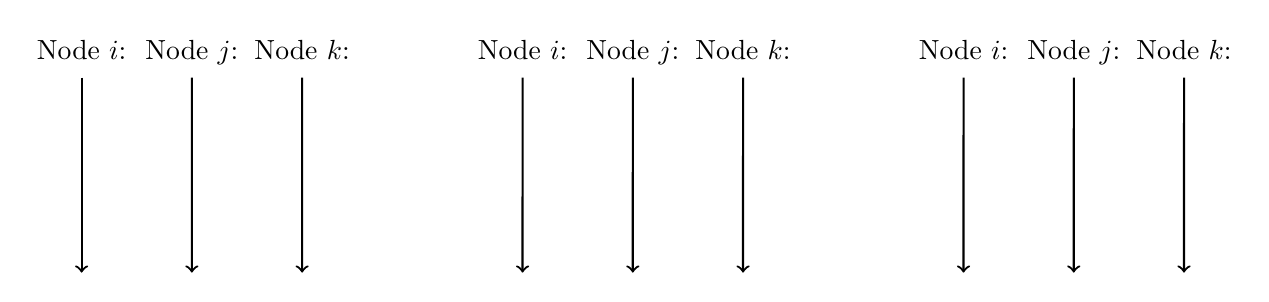
\begin{tikzpicture}[auto,scale=1.4]

\tikzstyle{every node}=[text height=8pt,text depth=3pt]
\tikzstyle{every path}=[thick,->]

\node (i1name) at (0,2) {Node $i$:};
\node (j1name) at (1,2) {Node $j$:};
\node (k1name) at (2,2) {Node $k$:};
\draw (i1name) -- (0,0);
\draw (j1name) -- (1,0);
\draw (k1name) -- (2,0);

\node (i2name) at (4,2) {Node $i$:};
\node (j2name) at (5,2) {Node $j$:};
\node (k2name) at (6,2) {Node $k$:};
\draw (i2name) -- (4,0);
\draw (j2name) -- (5,0);
\draw (k2name) -- (6,0);

\node (i3name) at (8,2) {Node $i$:};
\node (j3name) at (9,2) {Node $j$:};
\node (k3name) at (10,2) {Node $k$:};
\draw (i3name) -- (8,0);
\draw (j3name) -- (9,0);
\draw (k3name) -- (10,0);

\end{tikzpicture}

\caption{Illustrating the happens-before relation}\label{fig.happens-before}
\end{figure}

Figure~\ref{fig.happens-before} illustrates these three cases, and the formalisation of this
definition appears in Section~\ref{sect.network}.

In practice, the happens-before relationship can be captured using vector timestamps
\cite{Schwarz:1994gl,Fidge:1988tv,Raynal:1996jl}, which are used to implement protocols for causally
ordered delivery \cite{Cachin:2011wt}. As these protocols are widely known and well understood, we
leave them out of scope for this paper.


% Total order broadcast ensures that when nodes broadcast a set of messages to other nodes on the
% network, they are delivered in the same order to all recipients. By contrast, causal ordering is a
% weaker guarantee that allows greater concurrency and thus greater nondeterminism in the network.
% However, it has the advantage that it makes no assumptions about the number of nodes that are
% online.

% TODO happens-before


% There are two families of algorithms for collaborative editing: \emph{operational transformation}
% (OT)~\cite{Ellis:1989ue,Ressel:1996wx,Oster:2006tr,Sun:1998vf,Sun:1998un,Suleiman:1998eu,Nichols:1995fd}
% and \emph{conflict-free replicated datatypes}
% (CRDTs)~\cite{Shapiro:2011wy,Roh:2011dw,Preguica:2009fz,Oster:2006wj,Weiss:2010hx,Nedelec:2013ky,Kleppmann:2016ve}.
% Both allow a document to be modified concurrently on different replicas, with changes applied
% immediately to the local copy, while asynchronously propagating changes to other replicas. The
% goal of these algorithms is to ensure that for all concurrent executions, the replicas converge
% toward the same state without any edits being lost, a property known as \emph{strong eventual
% consistency}~\cite{Shapiro:2011un}.


% CRDTs are a more recent development~\cite{Shapiro:2011un}. While OT is based on transforming
% non-commutative operations so that they have the same effect when reordered, CRDTs define operations
% in a way that makes them commutative by design, making them more amenable to peer-to-peer settings
% in which each node may apply edits in a different order. CRDTs also have attractive performance
% characteristics~\cite{Mehdi:2011ke}.

% TODO Various decentralised algorithms have been proposed and all but one (Oster 2006) have
% subsequently been shown to be incorrect.

\begin{figure}
\centering
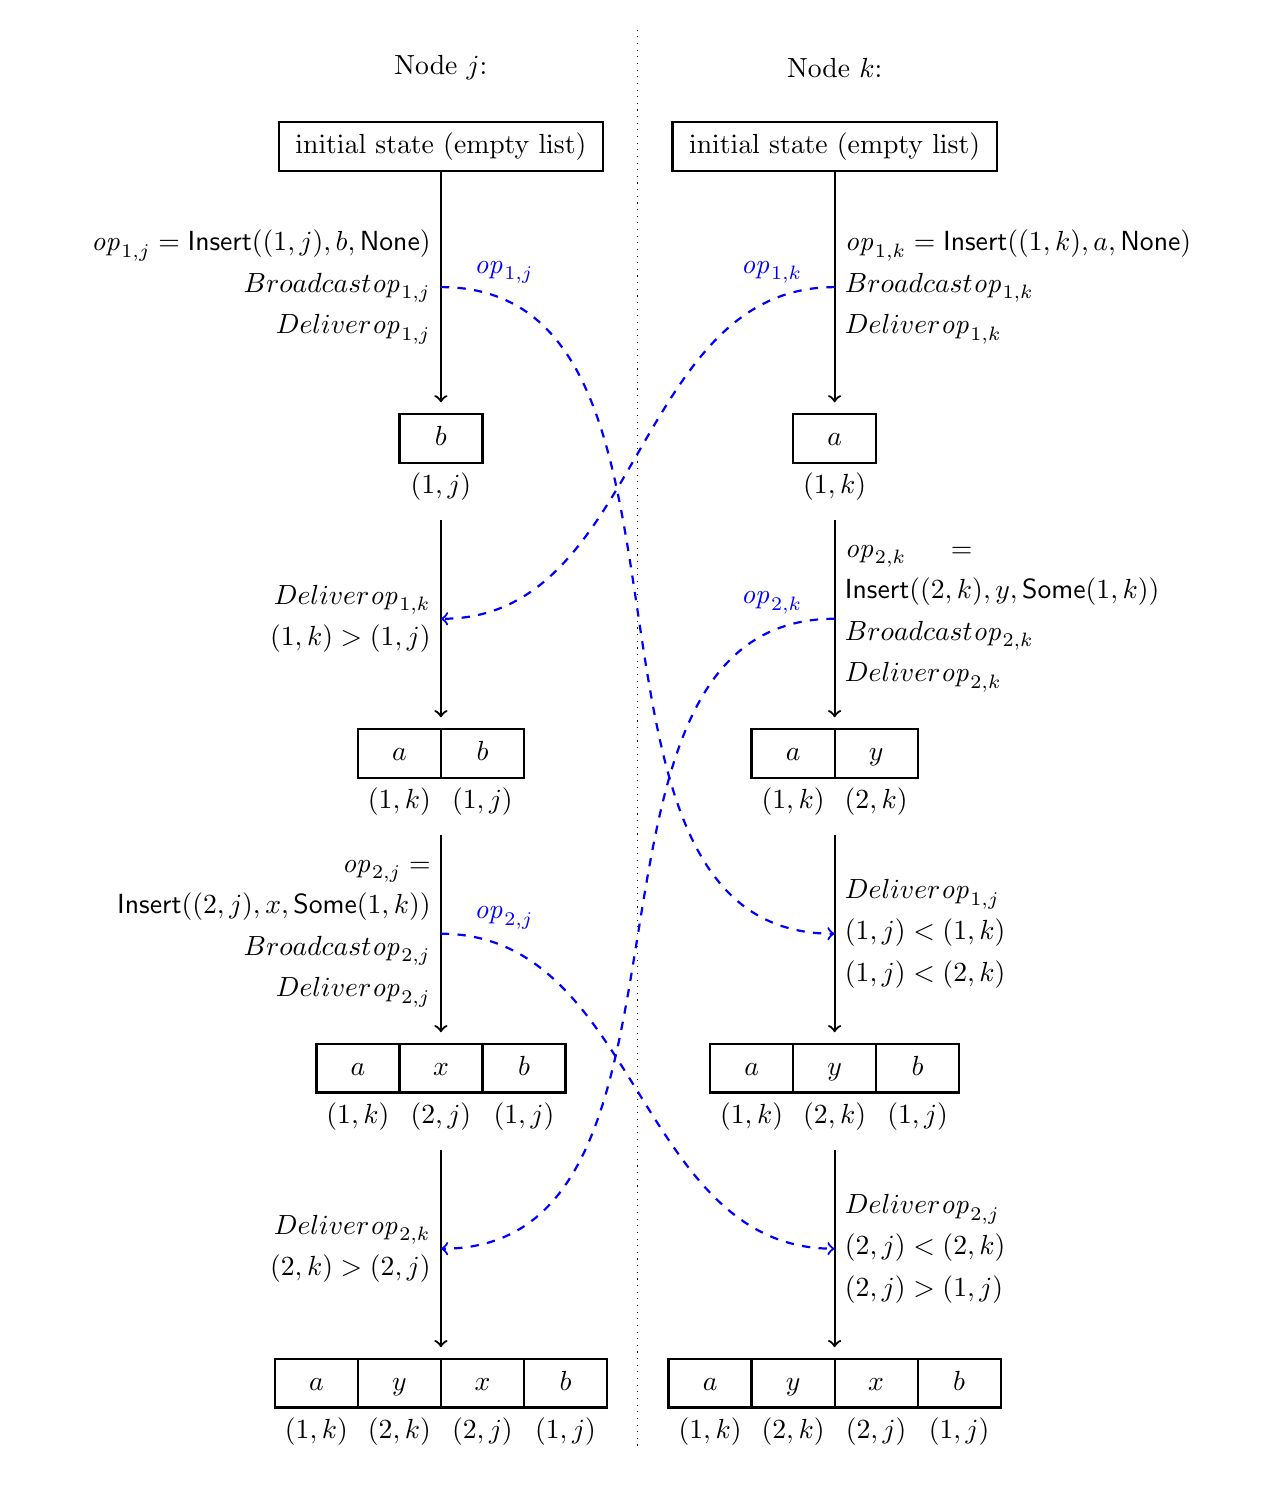
\begin{tikzpicture}[auto,scale=1.0]
\onehalfspacing
\path [draw,dotted] (2.5,-0.5) -- (2.5,17.5);

\tikzstyle{initstate}=[rectangle,draw,inner xsep=6pt,text height=8pt,text depth=3pt]
\tikzstyle{state}=[matrix,column sep={30pt,between origins}]
\tikzstyle{val}=[draw,anchor=base,minimum width=30pt,text height=8pt,text depth=3pt]
\tikzstyle{oid}=[anchor=base]
\tikzstyle{leftevent}=[left,text width=5cm,text ragged left,midway]
\tikzstyle{rightevent}=[right,text width=5cm,text ragged,midway]
\tikzstyle{every path}=[thick,->]

\node (leftR) at (0,17) {Node $j$:};
\node (left1) at (0,16) [initstate] {initial state (empty list)};
\node (left2) at (0,12) [state] {
    \node [val] {$b$};     \\
    \node [oid] {$(1,j)$}; \\
};
\node (left3) at (0,8) [state] {
    \node [val] {$a$};     & \node [val] {$b$};     \\
    \node [oid] {$(1,k)$}; & \node [oid] {$(1,j)$}; \\
};
\node (left4) at (0,4) [state] {
    \node [val] {$a$};     & \node [val] {$x$};     & \node [val] {$b$};     \\
    \node [oid] {$(1,k)$}; & \node [oid] {$(2,j)$}; & \node [oid] {$(1,j)$}; \\
};
\node (left5) at (0,0) [state] {
    \node [val] {$a$};     & \node [val] {$y$};     & \node [val] {$x$};     & \node [val] {$b$};     \\
    \node [oid] {$(1,k)$}; & \node [oid] {$(2,k)$}; & \node [oid] {$(2,j)$}; & \node [oid] {$(1,j)$}; \\
};

\draw (left1) -- (left2) node (send1j) [leftevent] {
    \hfill $\mathit{op}_{1,j} = \mathsf{Insert}((1, j), b, \mathsf{None})$ \\
    \hfill $\text{Broadcast } \mathit{op}_{1,j}$ \\
    \hfill $\text{Deliver } \mathit{op}_{1,j}$ \\
};
\draw (left2) -- (left3) node (recv1k) [leftevent] {
    \hfill $\text{Deliver } \mathit{op}_{1,k}$ \\
    \hfill $(1,k) > (1,j)$ \\
};
\draw (left3) -- (left4) node (send2j) [leftevent] {
    \hfill $\mathit{op}_{2,j} = \mathsf{Insert}((2, j), x, \mathsf{Some}(1,k))$ \\
    \hfill $\text{Broadcast } \mathit{op}_{2,j}$ \\
    \hfill $\text{Deliver } \mathit{op}_{2,j}$ \\
};
\draw (left4) -- (left5) node (recv2k) [leftevent] {
    \hfill $\text{Deliver } \mathit{op}_{2,k}$ \\
    \hfill $(2,k) > (2,j)$ \\
};

\node (rightR) at (5,17) {Node $k$:};
\node (right1) at (5,16) [initstate] {initial state (empty list)};
\node (right2) at (5,12) [state] {
    \node [val] {$a$};     \\
    \node [oid] {$(1,k)$}; \\
};
\node (right3) at (5,8) [state] {
    \node [val] {$a$};     & \node [val] {$y$};     \\
    \node [oid] {$(1,k)$}; & \node [oid] {$(2,k)$}; \\
};
\node (right4) at (5,4) [state] {
    \node [val] {$a$};     & \node [val] {$y$};     & \node [val] {$b$};     \\
    \node [oid] {$(1,k)$}; & \node [oid] {$(2,k)$}; & \node [oid] {$(1,j)$}; \\
};
\node (right5) at (5,0) [state] {
    \node [val] {$a$};     & \node [val] {$y$};     & \node [val] {$x$};     & \node [val] {$b$};     \\
    \node [oid] {$(1,k)$}; & \node [oid] {$(2,k)$}; & \node [oid] {$(2,j)$}; & \node [oid] {$(1,j)$}; \\
};

\draw (right1) -- (right2) node (send1k) [rightevent] {
    $\mathit{op}_{1,k} = \mathsf{Insert}((1, k), a, \mathsf{None})$ \\
    $\text{Broadcast } \mathit{op}_{1,k}$ \\
    $\text{Deliver } \mathit{op}_{1,k}$ \\
};
\draw (right2) -- (right3) node (send2k) [rightevent] {
    $\mathit{op}_{2,k} = \mathsf{Insert}((2, k), y, \mathsf{Some}(1, k))$ \\
    $\text{Broadcast } \mathit{op}_{2,k}$ \\
    $\text{Deliver } \mathit{op}_{2,k}$ \\
};
\draw (right3) -- (right4) node (recv1j) [rightevent] {
    $\text{Deliver } \mathit{op}_{1,j}$ \\
    $(1,j) < (1,k)$ \\
    $(1,j) < (2,k)$ \\
};
\draw (right4) -- (right5) node (recv2j) [rightevent] {
    $\text{Deliver } \mathit{op}_{2,j}$ \\
    $(2,j) < (2,k)$ \\
    $(2,j) > (1,j)$ \\
};

\begin{scope}[dashed,blue]
    \tikzstyle{every node}=[text centered]
    \draw (send1j.east) to [out=0,in=180] (recv1j.west);
    \draw (send2j.east) to [out=0,in=180] (recv2j.west);
    \draw (send1k.west) to [out=180,in=0] (recv1k.east);
    \draw (send2k.west) to [out=180,in=0] (recv2k.east);
    \node at (0.8,14.4) {$\mathit{op}_{1,j}$};
    \node at (0.8, 6.2) {$\mathit{op}_{2,j}$};
    \node at (4.2,14.4) {$\mathit{op}_{1,k}$};
    \node at (4.2,10.2) {$\mathit{op}_{2,k}$};
\end{scope}
\end{tikzpicture}

\caption{RGA example}\label{fig.two-lists}
\end{figure}


%%%%%%%%%%%%%%%%%%%%%%%%%%%%%%%%%%%%%%%%%%%%%%%%%%%%%%%%%%%%%%%%%%%%%%%%%%%%%%%%
% RGA_Network
%%%%%%%%%%%%%%%%%%%%%%%%%%%%%%%%%%%%%%%%%%%%%%%%%%%%%%%%%%%%%%%%%%%%%%%%%%%%%%%%

\section{Conclusion}
\label{sect.conclusion}

\subsection*{Acknowledgements}

\bibliography{references}{}

\end{document}
